\documentclass[]{article}
%\usepackage[a4paper, total={6.5in, 8.5in}]{geometry}
\usepackage{color}
\usepackage{hyperref}
\usepackage{amsmath}
\usepackage{amssymb}
\usepackage{graphicx}
\usepackage{wrapfig}
\usepackage{float}
\usepackage{algorithm}
\usepackage[noend]{algpseudocode}
\usepackage{neurips_data_2023}

\newcommand{\R}{\mathbb{R}}
\newcommand{\EE}{\mathbb{E}}
\newcommand{\N}{\mathbb{N}}
\newcommand{\D}{\mathcal{D}}
\newcommand{\X}{\mathcal{X}}
\newcommand{\Y}{\mathcal{Y}}
\newcommand{\U}{\mathcal{U}}
\newcommand{\LL}{\mathcal{L}}
\newcommand{\test}{\text{test}}
\newcommand{\train}{\text{train}}

\title{Towards Comparable Active Learning}
\author{%
	Anonymous Authors
	%Thorben Werner 
	%\thanks{Institute of Computer Science - Information Systems and Machine Learning Lab (ISMLL)} 
	%\\
	%University of Hildesheim\\
	%Universitätsplatz 1\, 31141 Hildesheim \\
	%\texttt{werner@ismll.de} \\
	% examples of more authors
	%\And
	%Johannes Burchert$^*$ \\
	%University of Hildesheim\\
	%Universitätsplatz 1, 31141 Hildesheim \\
	%\texttt{burchert@ismll.de} \\
	%\AND
	%Prof. Lars Schmidt-Thieme$^*$ \\
	%University of Hildesheim\\
	%Universitätsplatz 1, 31141 Hildesheim \\
	%\texttt{schmidt-thieme@ismll.uni-hildesheim.de}
}

\begin{document}

\maketitle

\begin{abstract}
	Active Learning has received significant attention in the field of machine learning for its potential in selecting the most informative samples for labeling, thereby reducing data annotation costs. However, the lack of reproducibility of performance gains reported in recent literature has created a chaotic landscape in Active Learning research. 
	This paper addresses these issues of inconsistent results in active learning (AL) literature.
	%Previous papers are constantly reporting significant performance improvements, while subsequent literature fails to reproduce those results. This inconsistency leads to a chaotic landscape of AL algorithms.
	To the best of our knowledge, we propose the first AL benchmark that tests algorithms in 3 major domains: Tabular, Image and Text.
	Furthermore, we highlight overlooked problems for reproducing AL experiments that can lead to unfair comparisons and increased variance in the results.
	To tackle these challenges, we propose an experimental protocol to accurately control the experiments.
	We report empirical results for 6 widely used algorithms on 7 datasets and aggregate them into a domain-specific ranking of AL algorithms.
\end{abstract}

\section{Introduction}
Deep neural networks (NN) have produced state-of-the-art results on many important supervised learning tasks.
Since Deep NNs usually require large amounts of labeled training data, Active Learning (AL) can be used to instead to select the most informative samples out of a large pool of unlabeled data, so that only these samples need to be labeled.
It has been shown that a small labeled set of this nature can be used to train well-performing models \cite{beck2021effective, hu2021towards, li2022empirical, zhou2021towards}. \\
%On top of providing a principled way to labeled unlabeled datasets, active learning is one of the two major approaches besides semi-supervised learning to make deep learning models more data efficient by requiring only a limited set of manually labeled data.
%Both approaches are at their core orthogonal and can freely be combined and therefore we should continue our research efforts for both approaches. \\
In the last decade many different algorithms for AL have been proposed.
Even though, almost every method has reported lifts all it's predecessors 
\footnote{out of all considered algorithms for this paper, only BALD \cite{gal2017deep} did not claim a new SOTA performance in their result section}
, AL research faces two central difficulties:
(i) The experiments are often carried out on different datasets and model architectures, hindering direct comparison,
(ii) the reported results prove to be very difficult to reproduce.
While multiple benchmark suites have been proposed to solve (i), to the best of our knowledge, we are the first to compare AL algorithms on all 3 data domains of vector, image and text.
Regarding (ii), \cite{zhou2021towards} has pointed out severe inconsistencies in results of AL papers in recent years. 
They conducted a meta analysis of reported results of several different AL algorithms and found that all considered algorithms only provided significant lifts in their own original papers, while following literature reported performances no better that uncertainty sampling, or in some cases no better than random sampling for the same algorithm (\cite{zhou2021towards} Appendix A).
The result of these inconsistencies is a chaotic landscape of AL algorithms where every paper claims to archive state-of-the-art performance
%by significantly outperforming everyone else
, while the vast majority of results proves to be non-reproducible. \\
In this work we propose an evaluation protocol that was designed to cope with the high variance in the performances of AL algorithms as well as being fully controllable regardless of the combination of dataset, model and AL algorithm.\\
We focus our work on single-sample pool-based AL where a pool of unlabeled samples is fixed at the start of each experiment and samples are chosen sequentially.
Specifically, we are not experimenting on so-called batch Active Learning, where at each iteration multiple unlabeled samples are chosen at the same time.
Even though most proposed algorithms (and benchmarks) are batched, they do not have a principled advantage over single-sample AL except speed of computation.
The problem of optimizing a portfolio of unlabeled samples in each iteration is more complicated to solve and the algorithms have systematically less information per sample to work with.
A performance comparison of batch AL and single-sample AL can be found in Fig. \ref{fig:ablation_bald}.
We can see that for two established algorithms BALD \cite{krizhevsky2009learning} and BADGE \cite{ashdeep} Batch AL can at most perform on-par with single-sample AL, independent of wether algorithm was originally designed for batch AL or not. \\
Table \ref{tab:benchmark_comparison} shows a feature comparison between our proposed benchmark and several existing benchmarks in the literature.
\begin{table}
	\centering
	\begin{tabular}{l | c c c c c}
		Paper & Sampling & \#Datasets & \#Domains & \#Algorithms & Oracle \\
		\hline
		Beck et al. \cite{beck2021effective} & batch & 4 & 1 & 7 & - \\
		Hu et al. \cite{hu2021towards} & batch & 5 & 2 & 13 & - \\
		Li et al. \cite{li2022empirical} & batch & 5 & 1 & 13 & - \\
		Zhou et al. \cite{zhou2021towards} & batch & 3 & 2 & 2 & \checkmark \\
		\textbf{Ours} & single & 7 & 3 & 6 & \checkmark 
	\end{tabular}
	\caption{Comparison of our benchmark with the existing literature. Oracle curves serve as an approximation of the best possible AL algorithm.}
	\label{tab:benchmark_comparison}
\end{table}

\subsection*{Contributions}
\begin{enumerate}
	\item Evaluation of Active Learning algorithms on datasets from 3 different domains
	\item Two novel synthetic dataset that highlight principled shortcomings of existing AL algorithms
	\item Novel experimental protocol for controlling AL experiments to allow full reproducibility
	\item Simple algorithm for an Oracle that can be constructed greedily and does not rely on search
\end{enumerate}


%%%%%%%%%%%%%%%%%%%%%%%%%%%%%%%%%%%%%%%%%%%%%%%%%%%%%%%%%%%%%%%%%%%%%%%%%%%%%%%%%%
\section{Problem Description}
Given two spaces $\mathcal{X}, \mathcal{Y}$, $n=l+u$ data points with $l \in \mathbb{N}$ labeled examples $\mathcal{L} = \{(x_1, y_1),\ldots, (x_l,y_l)\}$, $u \in \mathbb{N}$ unlabeled examples $\mathcal{U} = \{x_{l+1},\ldots,x_{n}\}$, a budget $\mathbb{N} \ni b \le u$ and an annotator $A: \mathbb{R}^\mathcal{X} \to \mathbb{R}^\mathcal{Y}$ that can label $x$. 
We call $x \in \mathcal{X}$, $y \in \mathcal{Y}$ predictors and labels respectively where $(x,y)$ are drawn from an unknown distribution $\rho$. 
Find an acquisition function $\Omega: \U^{(i)},\LL^{(i)} \mapsto x^{(i)}$ that iteratively selects the next unlabeled point $x^{(i)} \in \U^{(i)}$ for labeling
\begin{align*}
	\LL^{(i+1)} &\gets \LL^{(i)} \cup \{\left(x^{(i)}, A(x^{(i)})\right)\} \\
	\U^{(i+1)} &\gets \U^{(i)} \setminus x^{(i)} %, i \in 1{:}B
\end{align*}
so that the expected loss $\ell: \mathbb{R}^\mathcal{Y} \times \mathbb{R}^\mathcal{Y} \to \mathbb{R}$ of the machine learning algorithm $\hat y$ after $B$ iterations is minimal: 
$$\min \quad \mathbb{E}_{(x,y) \sim \rho} \ell(y, \hat{y}(\LL^{(B)}))$$
This formulation is a special case of the problem formulation in Appendix \ref{app:problem_formulation}.

\newpage
%%%%%%%%%%%%%%%%%%%%%%%%%%%%%%%%%%%%%%%%%%%%%%%%%%%%%%%%%%%%%%%%%%%%%%%%%%%%%%%%%%
%%%%%%%%%%%%%%%%%%%%%%%%%%%%%%%%%%%%%%%%%%%%%%%%%%%%%%%%%%%%%%%%%%%%%%%%%%%%%%%%%%
%%%%%%%%%%%%%%%%%%%%%%%%%%%%%%%%%%%%%%%%%%%%%%%%%%%%%%%%%%%%%%%%%%%%%%%%%%%%%%%%%%
\section{Related Work}
\begin{figure}
	\centering
	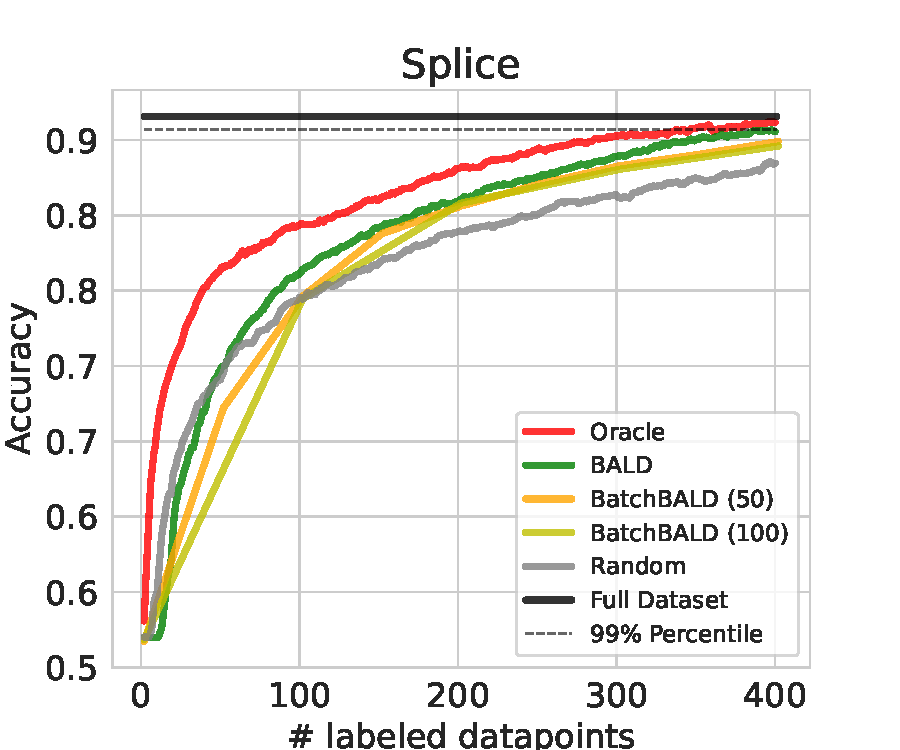
\includegraphics[width=0.49\linewidth]{img/ablation_splice_bald}
	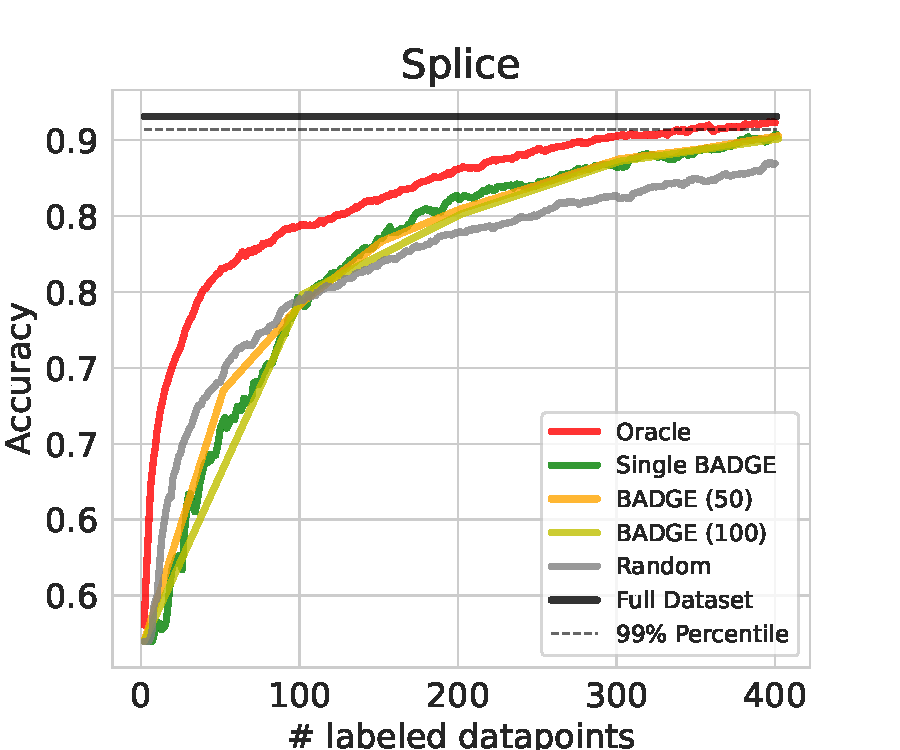
\includegraphics[width=0.49\linewidth]{img/ablation_splice_badge}
	\caption{Performance comparison of BALD \cite{gal2017deep} with it's batch AL adaptation \cite{kirsch2019batchbald} and BADGE \cite{ashdeep} with it's single-sample AL adaptation ($k=1$ in \cite{ashdeep} Alg. 1).
	In either scenario, the batched algorithm can at most perform on-par with it's single-sample analog, independent of wether it was originally designed for batch AL.}
	\label{fig:ablation_bald}
\end{figure}
Multiple benchmark suites have already been proposed for Active Learning:
The authors of \cite{beck2021effective} and \cite{li2022empirical} both focus exclusively on Batch AL in the image domain.
While \cite{beck2021effective} discuss a new metric to measure AL performance, which they call ``Label Efficiency'' and provide experiments on many common configurations of data preparation, model training and other hyperparameters, \cite{li2022empirical} focuses on combined approaches of AL and semi-supervised learning.
The authors of \cite{hu2021towards} study models that are trained with AL techniques in the image and text domain.
They test for several different properties of the models including robustness, response to compression techniques and final performance.
\cite{zhou2021towards} proposed an oracle algorithm for AL that uses Simulated Annealing search to approximate a solution for the optimal subset of labeled data.
Additionally, they study the generalization behavior of subsets of labeled data in the text an image domain.
The employed AL algorithms for our experiments are introduced in Section \ref{sec:sampling_strategies}.


%%%%%%%%%%%%%%%%%%%%%%%%%%%%%%%%%%%%%%%%%%%%%%%%%%%%%%%%%%%%%%%%%%%%%%%%%%%%%%%%%%
%%%%%%%%%%%%%%%%%%%%%%%%%%%%%%%%%%%%%%%%%%%%%%%%%%%%%%%%%%%%%%%%%%%%%%%%%%%%%%%%%%
%%%%%%%%%%%%%%%%%%%%%%%%%%%%%%%%%%%%%%%%%%%%%%%%%%%%%%%%%%%%%%%%%%%%%%%%%%%%%%%%%%
\section{Methodology}

%%%%%%%%%%%%%%%%%%%%%%%%%%%%%%%%%%%%%%%%%%%%%%%%%%%%%%%%%%%%%%%%%%%%%%%%%%%%%%%%%%
\subsection{Evaluation}\label{sec:evaluation}
Following \cite{zhou2021towards}, the quality of an AL algorithm is evaluated by an ``anytime" protocol that incorporates classification performance at every iteration, as opposed to evaluating final performance after the budget is exhausted.
We employ the normalized area under the accuracy curve (AUC):
\begin{equation}\label{eq:auc}
	\operatorname{AUC}(\mathcal{D}_{test}, \hat y, B) := \frac{1}{B} \sum_{i=1}^{B} \operatorname{Acc}(\mathcal{D}_{test}, \hat y_i)
\end{equation}
where $\hat y_i$ is the (re-)trained classification model after the i-\textit{th} iteration.
To mimic the leave-one-out protocol for cross-validation we will restart each experiment multiple times.
Each restart will retain the train/test split (often given by the dataset itself), but introduces a new validation split.
The AUC incorporates performance in early stages (low budget) as well as capabilities to push the classifier in later stages (high budget).
AL algorithms have to perform well in both scenarios. 
Since AL performance inhibits high variance and is prone to outliers, we propose to aggregate AUC values with their median instead of mean. \\ [1mm]
Since the AUC depends on the chosen budget, we need a general rule on how to set this hyperparameter that does not inherently benefit a subset of algorithms.
In this work, we choose the budget per dataset to be the first point at which any algorithm (except oracle) manages to reach a percentage of the upper bound performance measured on the full dataset.
Even though we would like to propose a single percentage value for all datasets, we found that different data modalities and use-cases need different percentages to produce sensible budgets
\footnote{Since we only consider single-sample AL, increasing the budget comes at a high computational cost. Therefore we could not freely increase the budget above 2000.}.
We propose the following values: \textbf{Tabular}: 99\%, \textbf{Image}: 90\%, \textbf{Text}: 95\%, \textbf{Embedded Data}: 90\%. \\ [1mm]
Additionally, we provide evidence in Fig. \ref{fig:restarts} that previous works have not evaluated their experiments with a sufficient number of restarts.
To create Fig. \ref{fig:restarts} we used 50 restarts from the margin/random acquisition function on the Splice dataset.
From these 50 runs we uniformly sampled subsets of runs and calculated the median AUC for this subset.
One of these median AUC values corresponds to one cross-validated experiment sampled from the distribution of experiments that are restarted exactly this many times.
To create one slice in Fig. \ref{fig:restarts}, we drew 50 samples from this distribution.
Each box-plot represents the variance of an evaluation if conducted with the respective number of restarts.
We can observe that low repetitions ($<10$) provide an uncertain evaluation where lucky and unlucky draws of the same experiment give drastically different median AUC values.
\begin{figure}
	\centering
	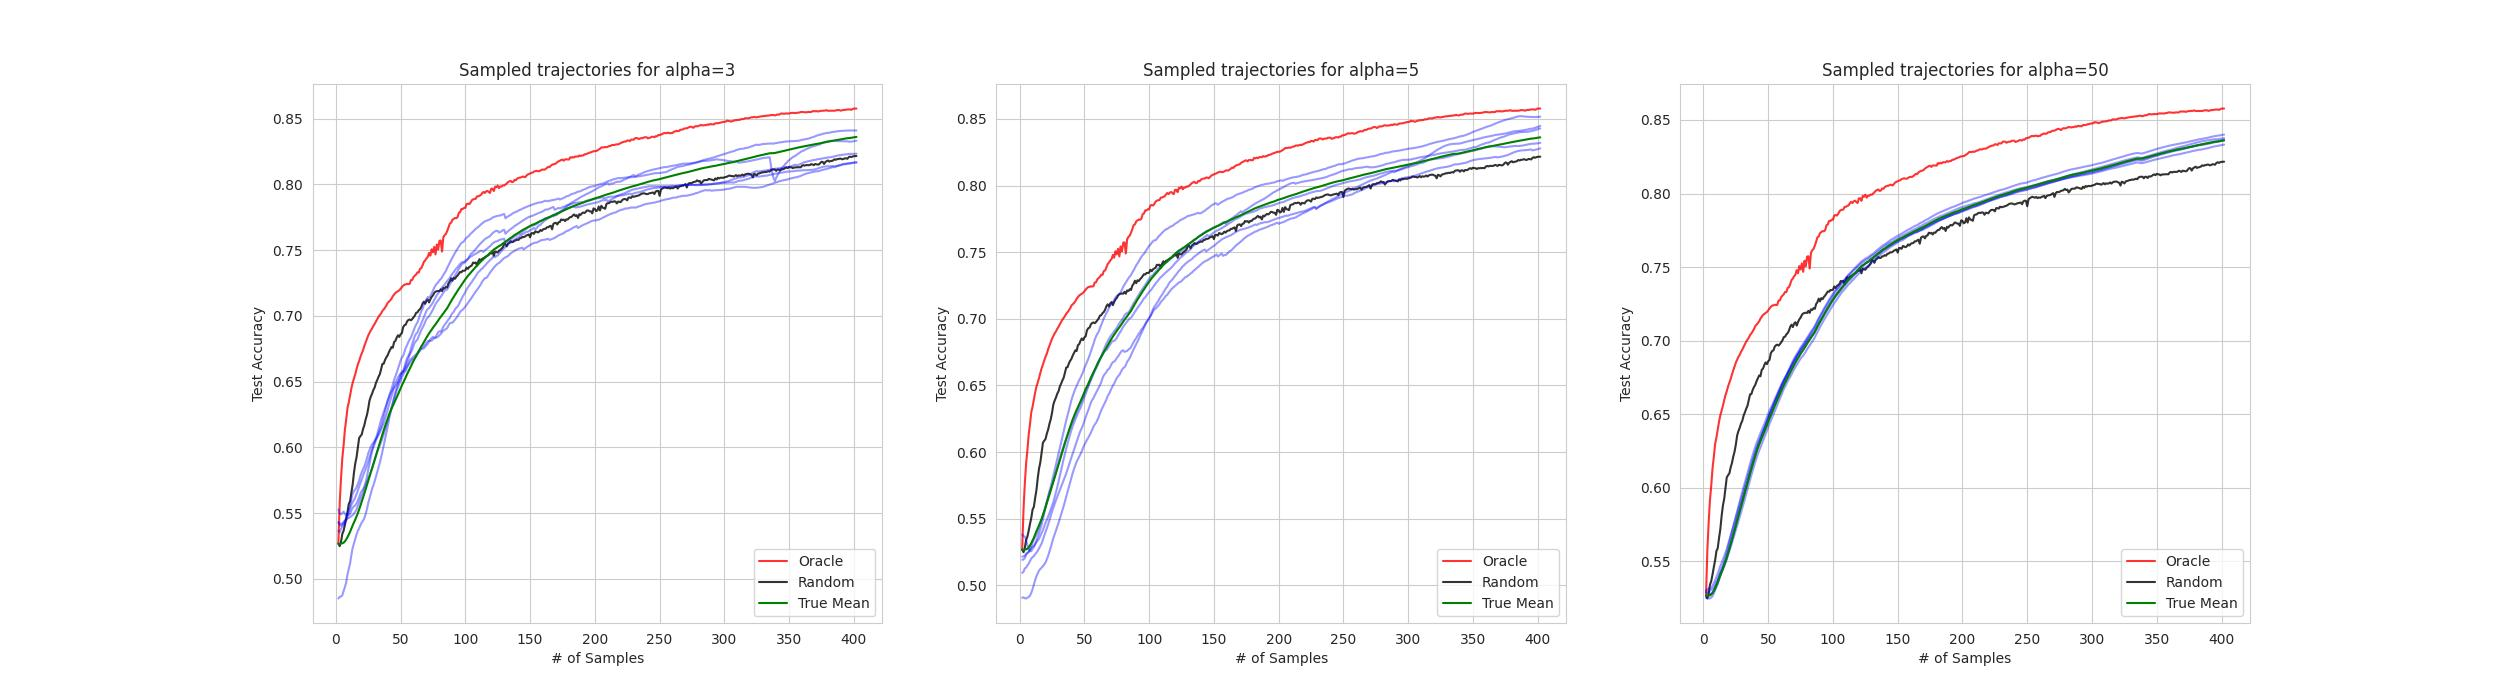
\includegraphics[width=\linewidth]{img/ablation_restarts}
	\caption{Random draws from an experimental distribution on the Splice dataset with different numbers of repetitions. Each point on the Y-axis represents a cross-validated result that could have been reported in a paper. This analysis shows the drastic differences in performance one could observe even when repeating an experiment 2-10 times.}
	\label{fig:restarts}
\end{figure}
To reliably arrive at the true median AUC, we propose to repeat every experiment 50 times, as only $>42$ repetitions don't produce outliers anymore (as indicated by the rightmost columns in Fig \ref{fig:restarts}).
One way to reduce the number of necessary repetitions would be to reduce the amount of variance in the experiment through specialized seeding (discussed in the next section).
We ultimately decided in favor of high variance and high number of repetitions as the high variance accurately reflects real world applications of AL.
%Fixing for example the classifier initialization to random draws from a constant seed does not have a corresponding use-case in the real world.


%%%%%%%%%%%%%%%%%%%%%%%%%%%%%%%%%%%%%%%%%%%%%%%%%%%%%%%%%%%%%%%%%%%%%%%%%%%%%%%%%%
\subsection{Reproducibility}\label{sec:reproducibility}
Previous works have noted adverse effects of training stochasticity on the evaluation of AL algorithms (\cite{zhou2021towards, lowell2018practical}).
Both papers observed that an actively sampled labeled set does not generalize well between model architectures or even different initializations of the same model.
To cater for this we aim to provide an experimental setup that is fully reproducible independent of the dataset, classification model or AL algorithm used.
For a fair comparison of two AL algorithms, both algorithms need to receive equal starting conditions in terms of train / validation split, initialization of classifier and even the state of minor systems like the optimizer or mini-batch sampler.
Even though different implementations might have their own solution to some of these problems, to the best of our knowledge no previous work has discussed this topic in detail.
The main obstacle for ensuring reproducibility is the seeding utility in PyTorch, Tensorflow and other frameworks, whose default choice is a single global seed.
Since many systems draw random numbers from this seed, all of them influence each other to a point where a single additional draw can completely change the model initialization or data split, depending on the ordering of these two in the implementation.
Even though some workarounds exists, like re-setting the seed multiple times, this problem is not limited to the initialization phase, but also extends to the AL iterations and the systems within.
We propose an implementation that creates a separate Random Number Generator (RNG) for each of these systems to ensure equal testing conditions even when the AL algorithm, dataset or classifier changes.
We hypothesize that the insufficient setup with global seeds contributes to the on-going problem of inconsistent results of AL algorithms in different papers. \\ [1mm]
In summary, we introduce three different seeds: $s_\Omega$ for the AL algorithm, $s_\mathcal{D}$ for dataset splitting and mini batch sampling and $s_\theta$ for model initialization and sampling of dropout masks.
Unless stated otherwise, we will keep $s_\Omega$ fixed for restarts of the same experiment, while $s_\mathcal{D}$ and $s_\theta$ are incremented by 1 between restarts to introduce stochasticity into our framework.
Some algorithms require a subsample to be drawn from $\mathcal{U}$ in order to reduce the computational cost in each iteration, while others need access to the full unlabeled pool (i.e. for effective clustering).
If a subsample is required, it will be drawn from $s_\Omega$ and therefore will not influence other systems in the experiments.
For each algorithm, we decided if subsampling is required based on our available hardware, but decided against setting a fixed time limit per experiment, since this would introduce unnecessary complexity into the benchmark.
An overview of selected hyperparameters per AL algorithm can be found in Appendix \ref{app:agent_hyperparameters}.

%%%%%%%%%%%%%%%%%%%%%%%%%%%%%%%%%%%%%%%%%%%%%%%%%%%%%%%%%%%%%%%%%%%%%%%%%%%%%%%%%%
\subsection{Oracle}\label{sec:oracle}
\begin{minipage}{0.5\linewidth}
	Posing Active Learning as a combinatorial problem, the oracle set $\mathcal{U}_b$ for a given dataset, model and training procedure is the set that induces the highest AUC score for a given budget.
	However, since this problem is not solvable for realistic datasets, previous works have proposed approximations to this oracle sequence. 
	\cite{zhou2021towards} has used simulated annealing to search for the optimal subset and used the best  solution found after a fixed time budget. 
	Even though their reported performance curves display a significant lift over all other algorithms, we found the computational cost of reproducing this oracle for all our datasets to be prohibitive (The authors reported the search to take several days per dataset on 8 V100 GPUs).
	In this paper we propose a greedy oracle algorithm that constructs an approximation of the optimal set in an iterative fashion.
\end{minipage}
\hspace{2mm}
\begin{minipage}{0.45\linewidth}
	\begin{algorithm}[H]
		\caption{Oracle}\label{alg:oracle}
		\begin{algorithmic}[1]
			\Require $\mathcal{U}, \mathcal{L}, \mathcal{Y}, \mathcal{D}_\text{test}$ Train, Margin, $\tau, \hat y_\theta$ 
			\State $\text{acc} \gets \operatorname{Train}(\mathcal{L}, \mathcal{D}_\text{test}, \hat y_\theta)$ 
			%\State $u \underset{\tau}{\sim} \text{unif}(1:|\mathcal{U}|)$
			\State $r^* \gets 0$
			\For{$k := 1 \ldots \tau$}
			\State $\mathcal{L}' \gets \mathcal{L}^{(i)} \cup \{(u_k, A(u_k))\}$
			\State $\text{acc}' \gets \operatorname{Train}(\mathcal{L}', \mathcal{D}_\text{test}, \hat y_\theta)$  
			\State $r \gets \text{acc} - \text{acc}'$
			\If{$r > r^*$} 
			\State $r^* \gets r$
			\State $u^* \gets u_k$
			\EndIf
			\EndFor
			\If{$r^* = 0$}
			\State $u^* \gets \operatorname{margin}(\mathcal{U}, \hat y_\theta)$
			\EndIf
			\Return $u^*$
		\end{algorithmic}
	\end{algorithm}
\end{minipage} \\ [1mm]
Our oracle simply evaluates every data point $u_k = \operatorname{unif(\mathcal{U} | k = 1 \ldots \tau)}$ in a subsample of unlabeled points by fitting the classifier $\hat y$ on $\mathcal{L}^{(i)} \cup u_k$ and directly measuring the resulting test performance.
The data point with the best test performance is selected and added to the labeled pool for that iteration.
We noticed that this oracle is overfitting on the test set, resulting in stagnating or even decreasing performance curves in later AL iterations.
This can happen for example, if the oracle picked a labeled set that enables the classifier to correctly classifier a big portion of easy samples in the test set, but now fails to find the next single unlabeled point that would enable the classifier to succeed on one of the hard samples in the test set.
This leads to a situation, where the selected data point is basically random.\\
To circumvent this problem, we introduced margin sampling \cite{wang2014new} as a fallback option for the oracle.
Whenever the oracle does not find an unlabeled point that results in an increase in performance, it defaults to margin sampling in that iteration.
The resulting greedy algorithm constructs an approximation of the optimal labeled set that consistently outperforms all other algorithms by a significant margin, while requiring relatively low computational cost (scaling linearly in $\tau$).
The pseudocode for our oracle can be found in Alg. \ref{alg:oracle}.
In the algorithm $\operatorname{Train}(\LL, \D_\text{test}, \hat y_\theta)$ trains the classification model $\hat y_\theta$ and returns it's accuracy  on $\D_\text{test}$. \\
Alg. \ref{alg:oracle} replaces the acquisition function in the AL process.


%%%%%%%%%%%%%%%%%%%%%%%%%%%%%%%%%%%%%%%%%%%%%%%%%%%%%%%%%%%%%%%%%%%%%%%%%%%%%%%%%%
\subsection{Sampling Strategies}\label{sec:sampling_strategies}
We selected AL algorithms that have good performances reported by multiple different sources.
To ensure a fair comparison, we fixed the training process of our classification model as well as the set of available information for the algorithms and selected only those that can work under these restrictions:\\
\textbf{Uncertainty Sampling} 
Tries to find the sample that the classifier is most uncertain about by computing heuristics of the class probabilities. For our benchmark we use entropy and margin (a.k.a. best-vs-second-best) sampling.\\
\textbf{BALD \cite{kirsch2019batchbald}}
Applies the query-by-committee strategy of model ensembles to a single model by interpreting the classifier's parameters as distributions and then sample multiple outputs from them via Monte-Carlo dropout.\\
\textbf{BADGE \cite{ashdeep}} Uses gradient embeddings of unlabeled points to select samples where the classifier is expected to change a lot. The higher the magnitude of the gradient the higher is the expected improvement in model performance.\\
\textbf{Coreset \cite{sener2017active}}
Employs K-Means clustering to try to cover the whole data distribution.
Selects the unlabeled sample that is the furthest away from all cluster centers.
Clustering is done in a semantically meaningful space by encoding the data with the current classifier $\hat y$.
In this work we use the greedy variant of Coreset.\\
\textbf{TypiClust \cite{hacohen2022active}}
Relies on clustering similar to Coreset but proposes a new measure called "Typicality" to select unlabeled samples.
Selects points that are in the densest regions of clusters that do not contain labeled samples yet.
Clustering is done in a semantically meaningful space by encoding the data with the current classifier $\hat y$.
It has to be pointed out that TypiClust was designed for low-budget scenarios, but we think it is still worthwhile to test and compare this algorithm with practically relevant budgets.
%
\subsubsection*{Honorable Mentions}
\textbf{Learning Loss for AL}
Introduces an updated training of the classification model with an auxiliary loss and therefore cannot be compared fairly against classification models without this boosted training regime.


%%%%%%%%%%%%%%%%%%%%%%%%%%%%%%%%%%%%%%%%%%%%%%%%%%%%%%%%%%%%%%%%%%%%%%%%%%%%%%%%%%
\subsection{Choosing the Classifier}\label{sec:choosing_the_classifier}
Traditionally, the classifier is chosen per dataset so that it is capable of solving the dataset close to the SOTA performance reported in the literature.
Since we are not interested in archiving a new SOTA in any classification problem, we opt to use smaller classifiers for the following reasons:
Smaller classifiers generally (i) exhibit more stable training behavior and (ii) on average require less sampled datapoints to reach the their upper bound performance on the full dataset.
For every dataset the chosen architecture's hyperparameters are optimized by to archive maximum upper bound performance.
One desired characteristic of these small classifiers is that the ranking of AL algorithms should stay the same when switching to larger models.
A small analysis of this behavior can be found in Appendix \ref{app:classifier_size}.
We found that the ranking of AL algorithms unfortunately does change slightly, but we did not observe systematics that benefit one or few specific algorithms.
We therefore rely on the different data domains to provide classification models of different sizes and archetypes to cover all of the use-cases.
For an overview of architectures and hyperparameters please refer to Appendix \ref{app:hyperparameters}.


%%%%%%%%%%%%%%%%%%%%%%%%%%%%%%%%%%%%%%%%%%%%%%%%%%%%%%%%%%%%%%%%%%%%%%%%%%%%%%%%%%
%%%%%%%%%%%%%%%%%%%%%%%%%%%%%%%%%%%%%%%%%%%%%%%%%%%%%%%%%%%%%%%%%%%%%%%%%%%%%%%%%%
\section{Implementation Details}
At each iteration $i$ the AL algorithm picks an unlabeled datapoint based on a fixed set of information $\{\mathcal{L}^{(i)}, \mathcal{U}^{(i)}, B, |\mathcal{L}^{(i)}|-|\mathcal{L}^{(1)}|, \text{acc}^{(i)}, \text{acc}^{(1)}, \theta^{(i)}, \text{opt}_\theta\}$, where $\theta^{(i)}$ is the current classifier and $\text{opt}_\theta$ is the optimizer used to fit $\theta^{(i)}$.
We allow algorithms to derive additional information of this set like predictions of the classifier, K-Means clustering or even training new classifiers.
However, the algorithm may not incorporate external information like other datasets, queries to recover additional labels, additional training steps for the classifier, or the test/validation set.

%%%%%%%%%%%%%%%%%%%%%%%%%%%%%%%%%%%%%%%%%%%%%%%%%%%%%%%%%%%%%%%%%%%%%%%%%%%%%%%%%%
\subsection{Training the Classifier}\label{sec:training_the_classifier}
The classification model can be trained in two ways. Either you reset the parameters after each AL iteration and train the classifier from scratch with the updated labeled set $\mathcal{L}^{(i)}$, or you retain the previous state and only fine-tune the classifier on $\mathcal{L}^{(i)}$ for a reduced number of epochs.
In this work we use the fine-tuning method for raw datasets to save computation, while we use the from-scratch training for embedded dataset, since they have very small classifiers and this method generally produces better results.
Our fine-tuning scheme always trains for at least one epoch and employs an aggressive early stopping after that.
The early stopping has patience 0, so it will stop as soon as the validation loss does no longer decrease.
Even though the use of a fully labeled validation set might be regarded as impractical, since such a set will never exist during deployment, we strongly advocate for using it in benchmarks to control the classifier training.
In this work we use the validation set to optimize the hyperparameters of the classifier and reduce overfitting with early stopping the training process in every iteration.

%%%%%%%%%%%%%%%%%%%%%%%%%%%%%%%%%%%%%%%%%%%%%%%%%%%%%%%%%%%%%%%%%%%%%%%%%%%%%%%%%%
%%%%%%%%%%%%%%%%%%%%%%%%%%%%%%%%%%%%%%%%%%%%%%%%%%%%%%%%%%%%%%%%%%%%%%%%%%%%%%%%%%
\section{Experiments}

%%%%%%%%%%%%%%%%%%%%%%%%%%%%%%%%%%%%%%%%%%%%%%%%%%%%%%%%%%%%%%%%%%%%%%%%%%%%%%%%%%
\subsection{Datasets}\label{sec:datasets}
For all our datasets we use the pre-defined train / test splits, if given. 
In the remaining cases, we define test sets upfront and store them into separate files to keep them fixed across all experiments.
The validation set is split during experiment-time and depends on the dataset-seed.\\
\textbf{Tabular:}
We use \textbf{Splice}, \textbf{DNA} and \textbf{USPS} from LibSVMTools \cite{libsvmtools}.
All three datasets are normalized between [0, 1]. \\
\textbf{Image:}
We use \textbf{FashionMNIST} \cite{xiao2017fashion} and \textbf{Cifar10} \cite{krizhevsky2009learning}.
Both datasets are normalized according to their standard protocols. \\
\textbf{Text:}
We use \textbf{News Category} \cite{misra2022news} and \textbf{TopV2} \cite{chen-etal-2020-low-resource}.
For News Category we use  the 15 most common categories as indicated by its Kaggle site.
We additionally drop sentences above 80 words to reduce the padding needed (retaining 99,86\% of the data).
For TopV2, we are only using the "alarm" domain.
Both datasets are encoded with pre-trained GloVe (Common Crawl 840B Tokens) embeddings \cite{pennington2014glove}.
Since neither dataset provided a fixed test set, we randomly split 7000 datapoints into a test set. \\ [1mm]
%
We would like to point out that these datasets can be considered "toy-datasets" and therefore not relevant for practical purposes.
This might be true if we aimed to develop novel classification models on these datasets, however, similar to our argumentation for picking smaller classifiers, we are solely focused on comparing different AL algorithms in this paper.
Our core assumption is that a well-performing algorithm in our benchmark will also transfer into more practical use-cases. \\ [1mm]
Adapting the experimental setting from \cite{hacohen2022active} we offer all our datasets in the raw setting as well as pre-encoded by a fixed embedding model that was trained by unsupervised contrastive learning. 
The text datasets are an exception, as they are only offered in their encoded form.
The pre-encoded datasets enable us to test our single-sample algorithms on more complex datasets like Cifar10 and FashionMnist without the need of sampling $>2000$ datapoints before we can reach our upper bound performance.
The embedding model was trained with the SimCLR \cite{chen2020simple} algorithm. 
For Cifar10 we adapt the reported hyperparameters from \cite{hacohen2022active} and for the tabular datasets we use random search to optimize the hyperparameters.
The quality of embeddings during pretext training was measured after each epoch by attaching a linear classification head and evaluating this classifier for test accuracy, mirroring our AL setup for embedded datasets.

%%%%%%%%%%%%%%%%%%%%%%%%%%%%%%%%%%%%%%%%%%%%%%%%%%%%%%%%%%%%%%%%%%%%%%%%%%%%%%%%%%
\subsection{Results}

%\begin{table}[]
%	\centering
%	\begin{tabular}{l|lll}
%		& Splice        & DNA           & USPS          \\
%		\hline
%		Oracle          & 0.830 +- 0.01 & 0.836 +- 0.02 & 0.823 +- 0.01 \\
%		SAL & 0.799 +- 0.01 & 0.797 +- 0.03 & 0.809 +- 0.01 \\
%		Coreset & 0.800 +- 0.01 & 0.795 +- 0.03 & 0.787 +- 0.02 \\
%		TypiClust       & 0.790 +- 0.01 & 0.771 +- 0.04 & 0.761 +- 0.02 \\
%		MarginScore     & 0.797 +- 0.02 & 0.795 +- 0.04 & 0.808 +- 0.01 \\
%		ShannonEntropy  & 0.799 +- 0.02 & 0.794 +- 0.04 & 0.807 +- 0.01 \\
%		RandomAgent     & 0.788 +- 0.01 & 0.765 +- 0.03 & 0.772 +- 0.01 \\
%		Badge           & 0.807 +- 0.01 & 0.769 +- 0.06 & 0.797 +- 0.02 \\
%		BALD            & 0.811 +- 0.01 & 0.743 +- 0.04 & 0.717 +- 0.05
%	\end{tabular}
%	\caption{Median AUC values and standard deviation for all algorithms on the tabular datasets. Higher is better.}
%\end{table}
%
\begin{figure}
	\centering
	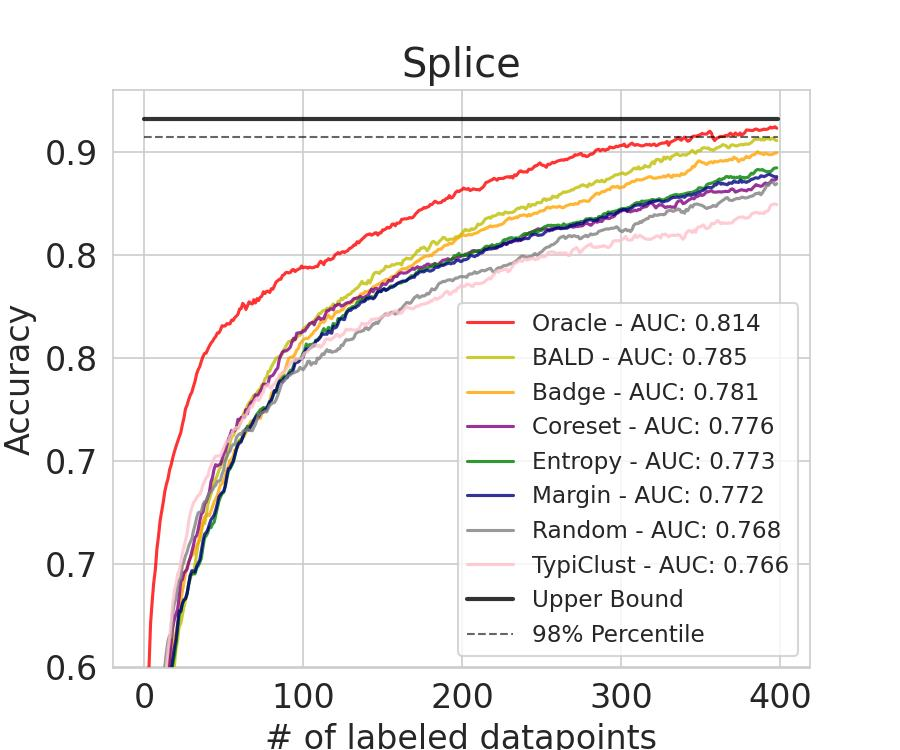
\includegraphics[width=0.49\linewidth]{img/eval_splice}
	\hspace{1mm}
	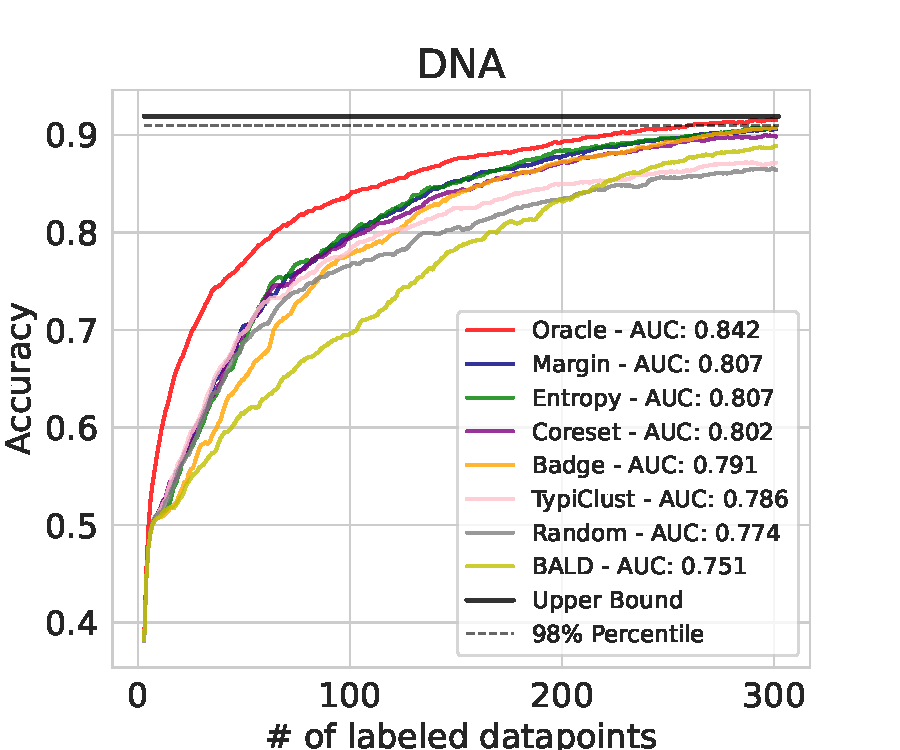
\includegraphics[width=0.49\linewidth]{img/eval_dna}\\[2mm]
	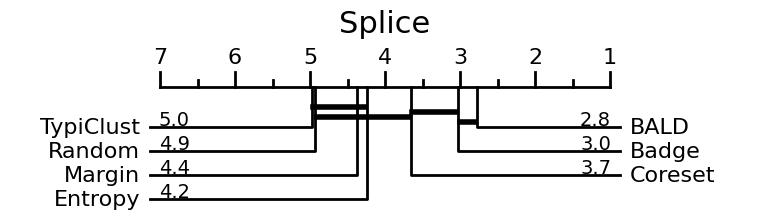
\includegraphics[width=0.49\linewidth]{img/micro_splice}
	\hspace{1mm}
	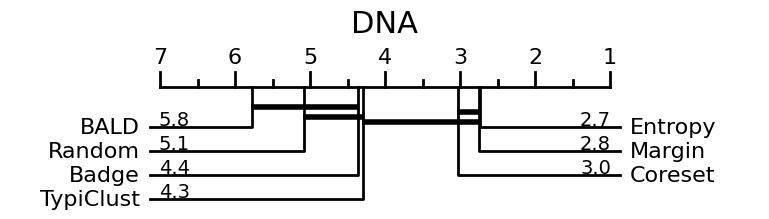
\includegraphics[width=0.49\linewidth]{img/micro_dna}
	\caption{Results for all algorithms on Splice and DNA, both from the tabular domain. Even within one domain, the performance of the same algorithm can vary drastically.}
	\label{fig:eval_vector}
\end{figure}
%
\begin{figure}
\centering
	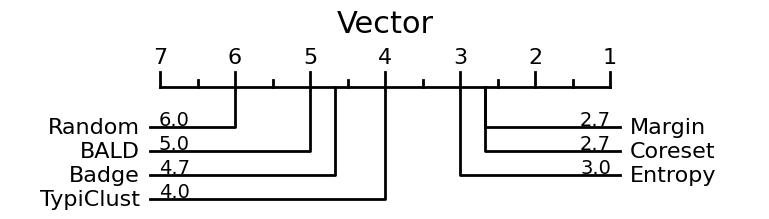
\includegraphics[width=0.49\linewidth]{img/macro_vector}
	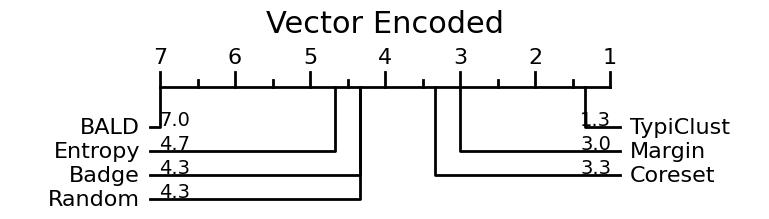
\includegraphics[width=0.49\linewidth]{img/macro_vector_enc}
	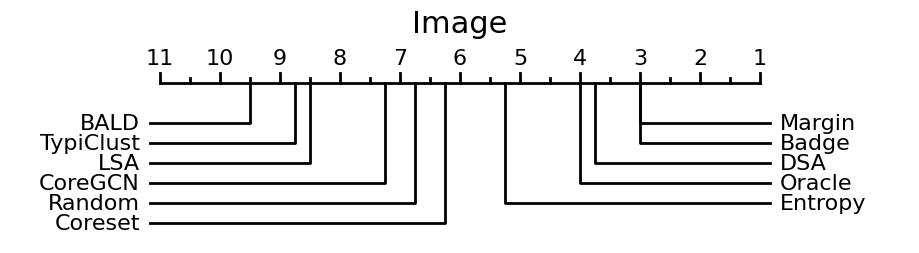
\includegraphics[width=0.49\linewidth]{img/macro_img}
	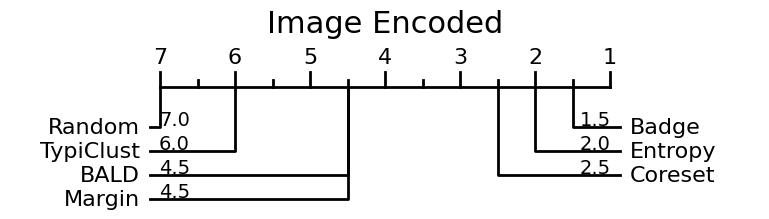
\includegraphics[width=0.49\linewidth]{img/macro_img_enc}
	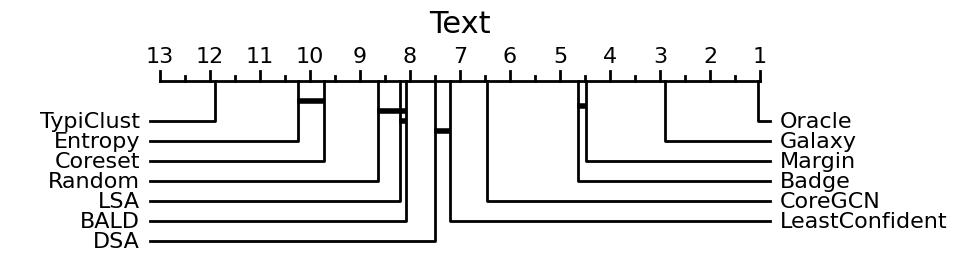
\includegraphics[width=0.49\linewidth]{img/macro_text}
	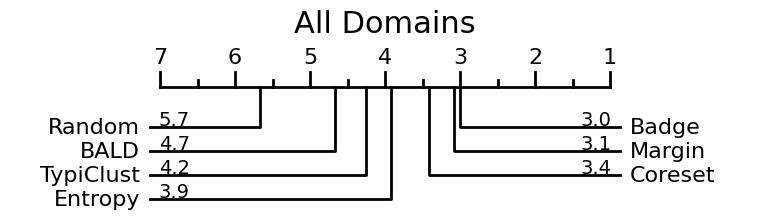
\includegraphics[width=0.49\linewidth]{img/macro_all.jpg}
	\caption{Critical Difference Diagram for all algorithms grouped by domain and all domains combined. Ranks are computed based on median AUC for each algorithm and dataset combination. Lower ranks are better.}
	\label{fig:cd_diagrams}
\end{figure}
%
From Fig. \ref{fig:eval_vector} we notice drastically different qualities for the same AL algorithm for different datasets.
We would like to highlight that both datasets are tabular from the medical domain with similar number of features and classes, yet we see that i.e. BALD is the best algorithm for Splice and the worst algorithm for DNA.
These inconsistencies are present between the datasets of all our tested domains, further highlighting the difficulties for comparing AL algorithms in terms of average performance.
In order to provide a meaningful analysis of which algorithm can be expected to perform best on average we ranked the algorithm for each dataset based on their median AUC and displayed these rankings in critical difference diagrams \cite{IsmailFawaz2018deep}.
In Fig. \ref{fig:cd_diagrams} we report the rankings split by domain as well as across all domains (excluding the toydata). \\ [2mm]
%
BALD performs bad with linear classifiers since they are trained without dropout and cannot cope well with missing inputs. \\
TypiClust is better with embedded data not only due to lower budgets. On other datasets it is not able to outperform other algorithms in early stages

% Missing:
% Seed set

\section{Discussion}
Domains are very different \\
Even within one domain we have stark differences (Fig. \ref{fig:eval_vector}) \\
Best 3 ranks for all domains are 3, 3.1 and 3.4 ... No clear winner \\
At least on average everything is better that random \\
BADGE: "Separately, we notice that diversity sampling only seems to work well when either the model has good architectural priors (inductive biases) built in, or when the data are easy to learn. Otherwise, penultimate layer representations are not meaningful, and diverse sampling can be deleterious. For this reason, CORESET often performs worse than random on sufficiently complex data when not using a convolutional network (Figure 3b)" \\

\section{Limitations and Future Work}
No batch AL \\
No learned algorithms \\
No SOTA classifier training (data augmentation, semi-supervised, etc.) \\
SimCRL as Pretext task works better for images

\newpage

\begin{ack}
	Funded by the Lower Saxony Ministry of Science and Culture under grant number ZN3492 within the Lower Saxony “Vorab“ of the Volkswagen Foundation and supported by the Center for Digital Innovations (ZDIN).
\end{ack}

\bibliographystyle{plain}
\bibliography{main.bib} 

\appendix

\section{Problem Formulation}\label{app:problem_formulation}
Given
\begin{itemize}
	\item a number $B\in\N$ (called budget),
	\item two spaces $\X$ and $\Y$,  {\tiny e.g., $\X:=\R^M, \Y:=\R^T$},
	\item a sample $\D_1,\ldots,\D_N \in (\X\times \Y)^*$ of
	sequences of pairs $(x,y)$  from an unknown distribution $p$
	(called datasets),
	%  {\tiny with $|\D_n|\geq B$ for all $n\in 1{:}N$,}
	{\tiny with $p(\D)=0$ for $|\D|<B$,}
	\item a function $\ell:\Y\times\Y\rightarrow\R$ (called loss), and
	\item a function $\hat y:  (\X\times \Y)^* \times \X^* \rightarrow \Y^\X$
	(called learning algorithm), \\
	{\tiny where $\Y^\X$ is the space of all function from $\X$ to $\Y$}
\end{itemize}
find a function
\vspace*{-0.5cm}
\begin{align*}
	\Omega: (\X\times \Y)^* \times \X^* &\rightarrow \N
	\quad\quad \text{\tiny (with $a(\D,X) \leq |X|$)} \\
	& \text{\tiny where $a(\D,X)$ selects an unlabeled instance from $X$}
\end{align*}
% which is equivariant in the second argument,

called acquisition function,
s.t. the expected loss of a model learned on all predictors plus $B$ sequentially acquired targets
is minimal:
\begin{align*}
	\min\ \EE\   &  \{
	% \operatorname{avg}\limits_{(x,y)\in\D\test} \ell(y, \hat y(x))
	\ell(\hat y, \D\test)
	\mid \D\sim p, (\D\train,\D\test):= \text{split}(\D) \}
	\\
	\text{with }
	\hat y:= & A( (\D_{\train_{n_1}},\ldots,\D_{\train_{n_B}}), \D\train|_{\X})
	\\ 
	n_b := & a( (\D_{\train_{n_1}},\ldots,\D_{\train_{n_{b-1}}}), \D\train|_{\X}) ,
	\quad b\in 1{:}B
\end{align*}

\section{All Results}\label{app:all_results}
\begin{figure}[H]
	\centering
	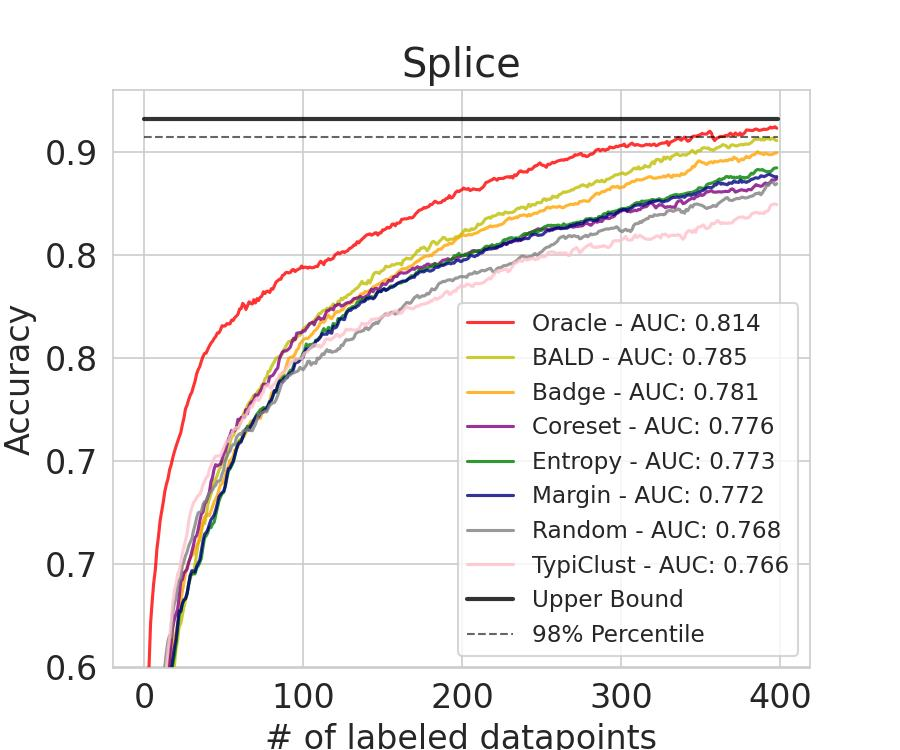
\includegraphics[width=0.49\linewidth]{img/eval_splice}
	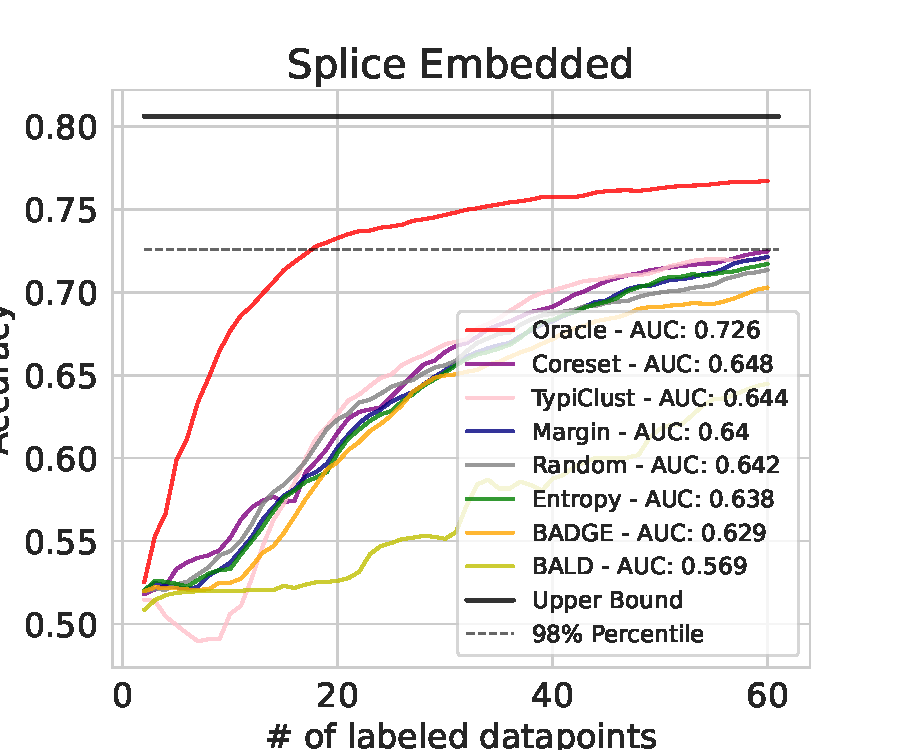
\includegraphics[width=0.49\linewidth]{img/eval_splice_enc} \\ [2mm]
	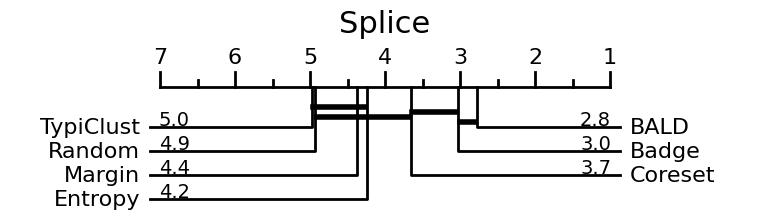
\includegraphics[width=0.49\linewidth]{img/micro_splice.jpg}
	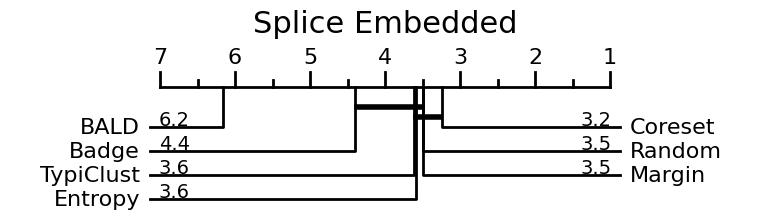
\includegraphics[width=0.49\linewidth]{img/micro_splice_enc.jpg} \\ [4mm]
\end{figure}
\begin{figure}[H]
	\centering
	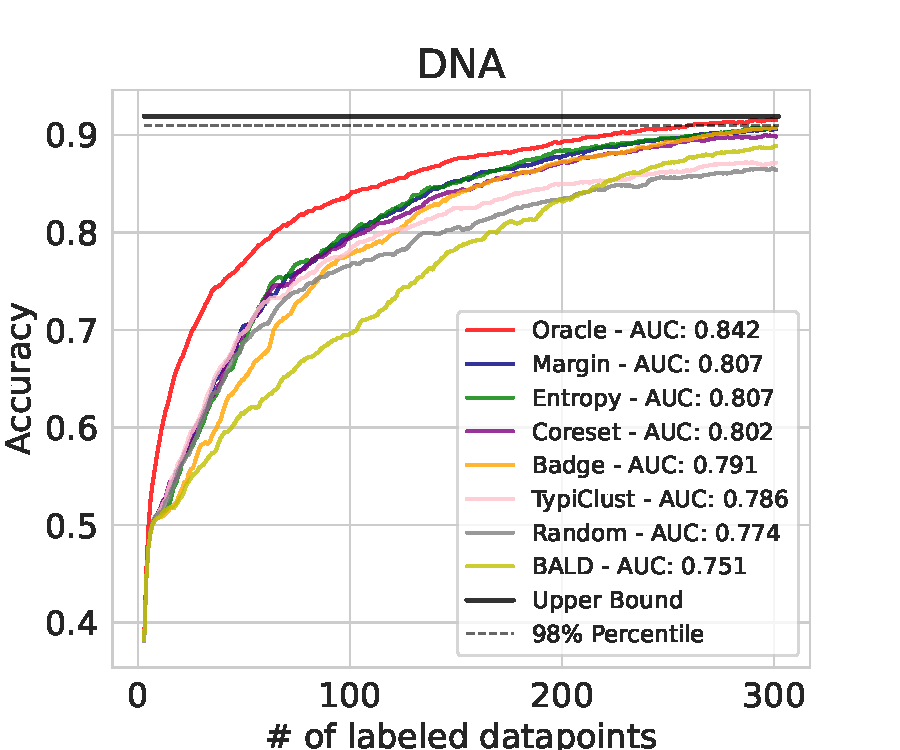
\includegraphics[width=0.49\linewidth]{img/eval_dna}
	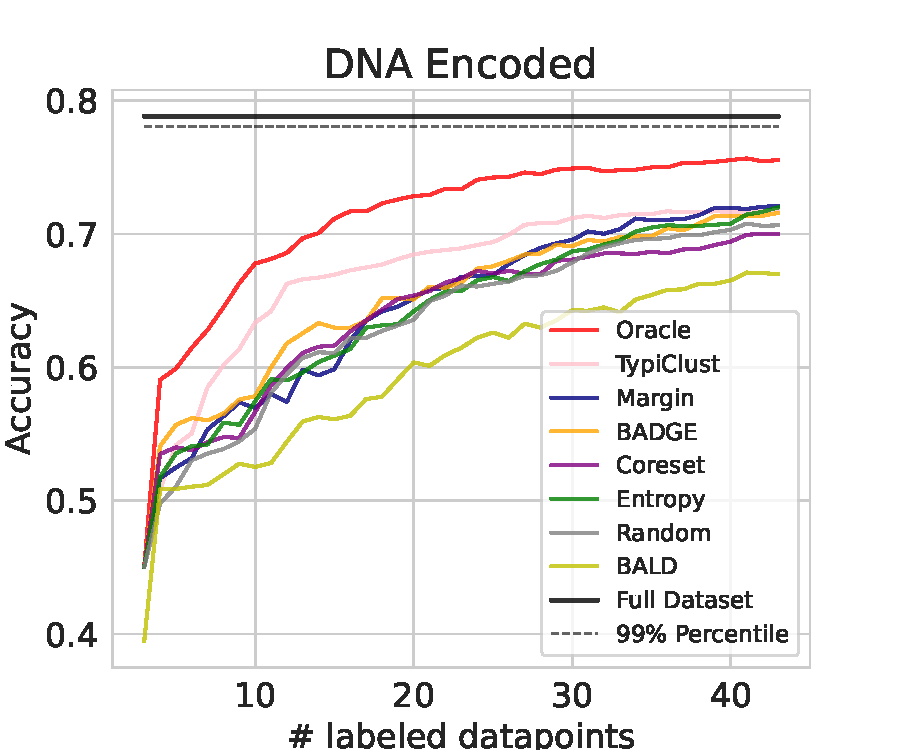
\includegraphics[width=0.49\linewidth]{img/eval_dna_enc} \\ [2mm]
	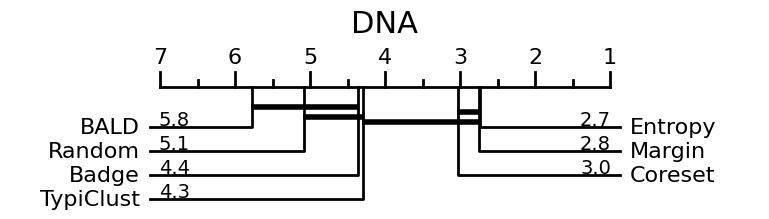
\includegraphics[width=0.49\linewidth]{img/micro_dna.jpg}
	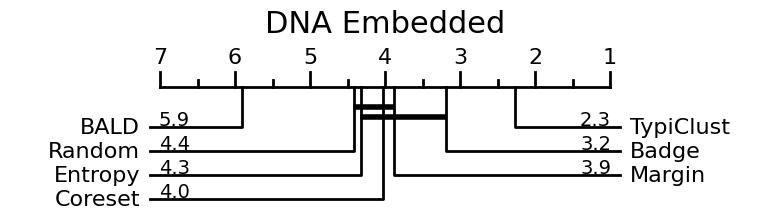
\includegraphics[width=0.49\linewidth]{img/micro_dna_enc.jpg} \\ [4mm]
\end{figure}
\begin{figure}[H]
	\centering
	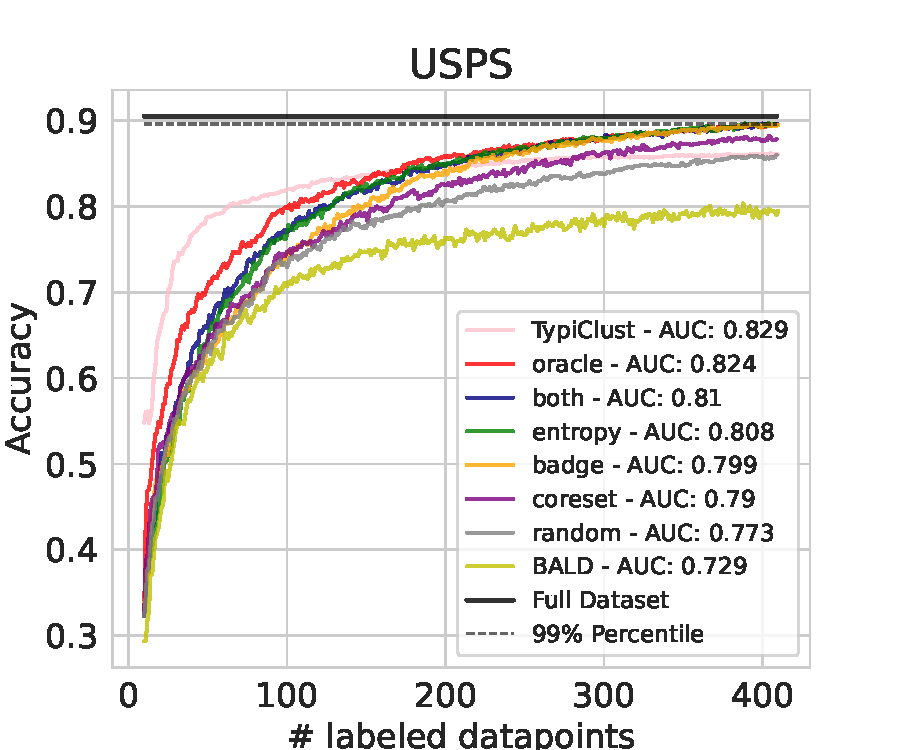
\includegraphics[width=0.49\linewidth]{img/eval_usps}
	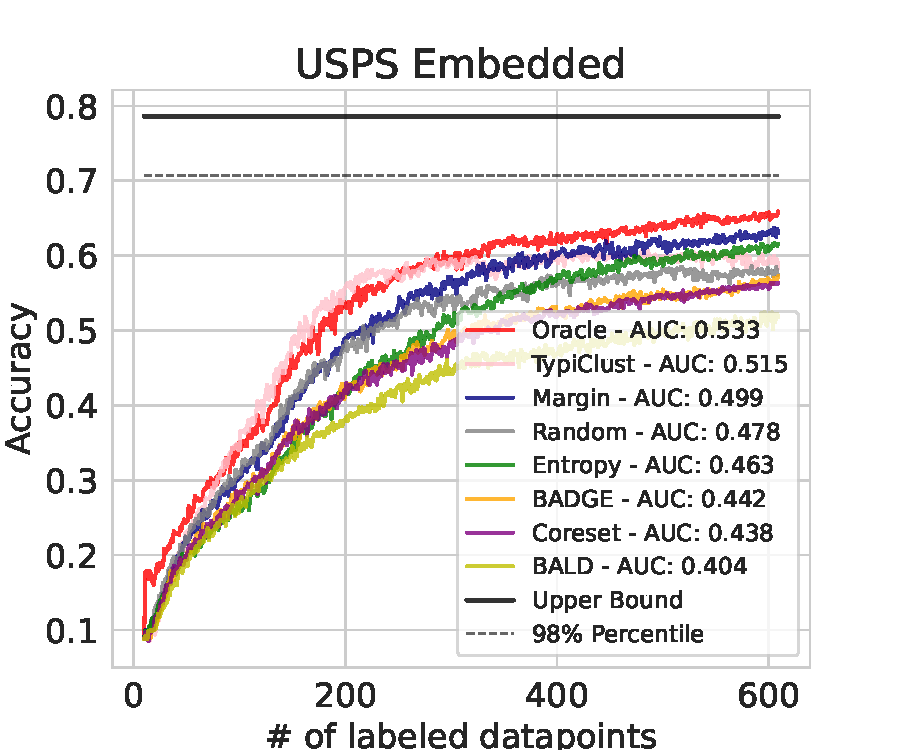
\includegraphics[width=0.49\linewidth]{img/eval_usps_enc} \\ [2mm]
	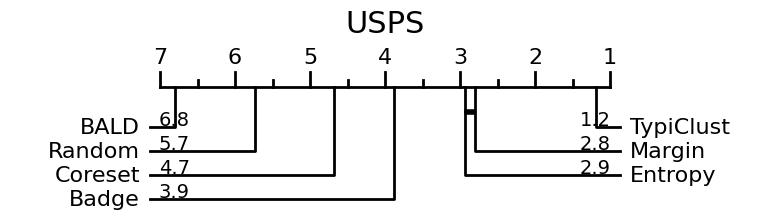
\includegraphics[width=0.49\linewidth]{img/micro_usps.jpg}
	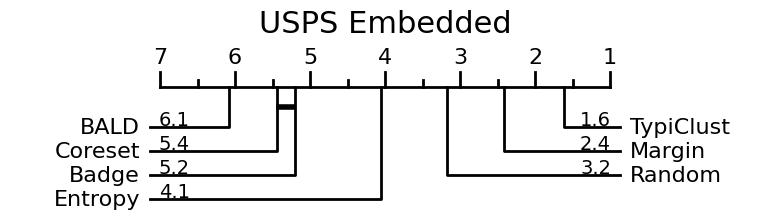
\includegraphics[width=0.49\linewidth]{img/micro_usps_enc.jpg} \\ [4mm]
\end{figure}
\begin{figure}[H]
\centering
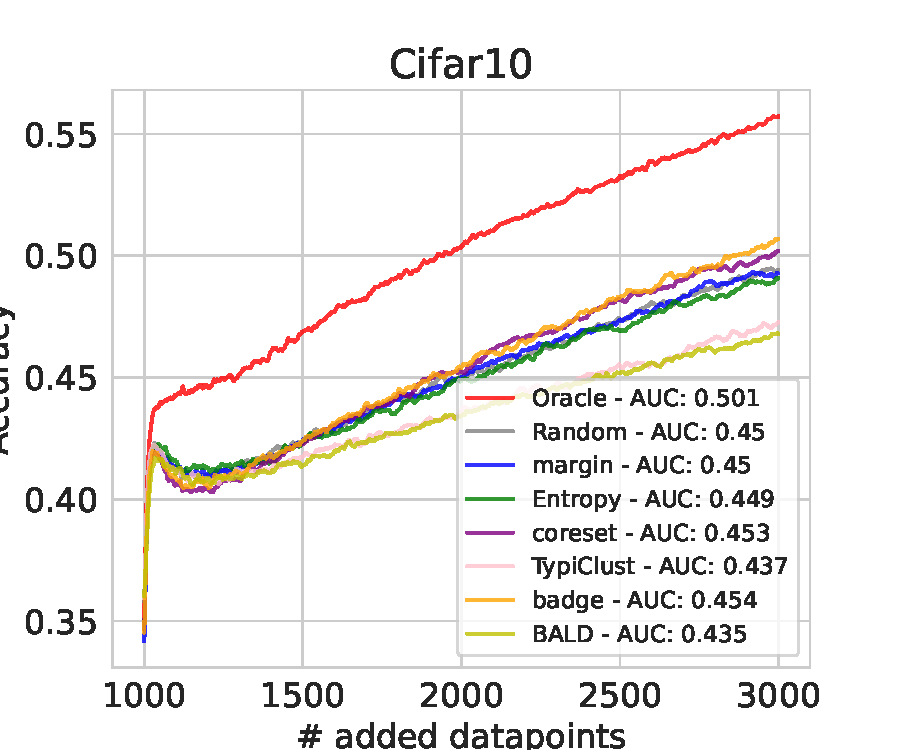
\includegraphics[width=0.49\linewidth]{img/eval_cifar10}
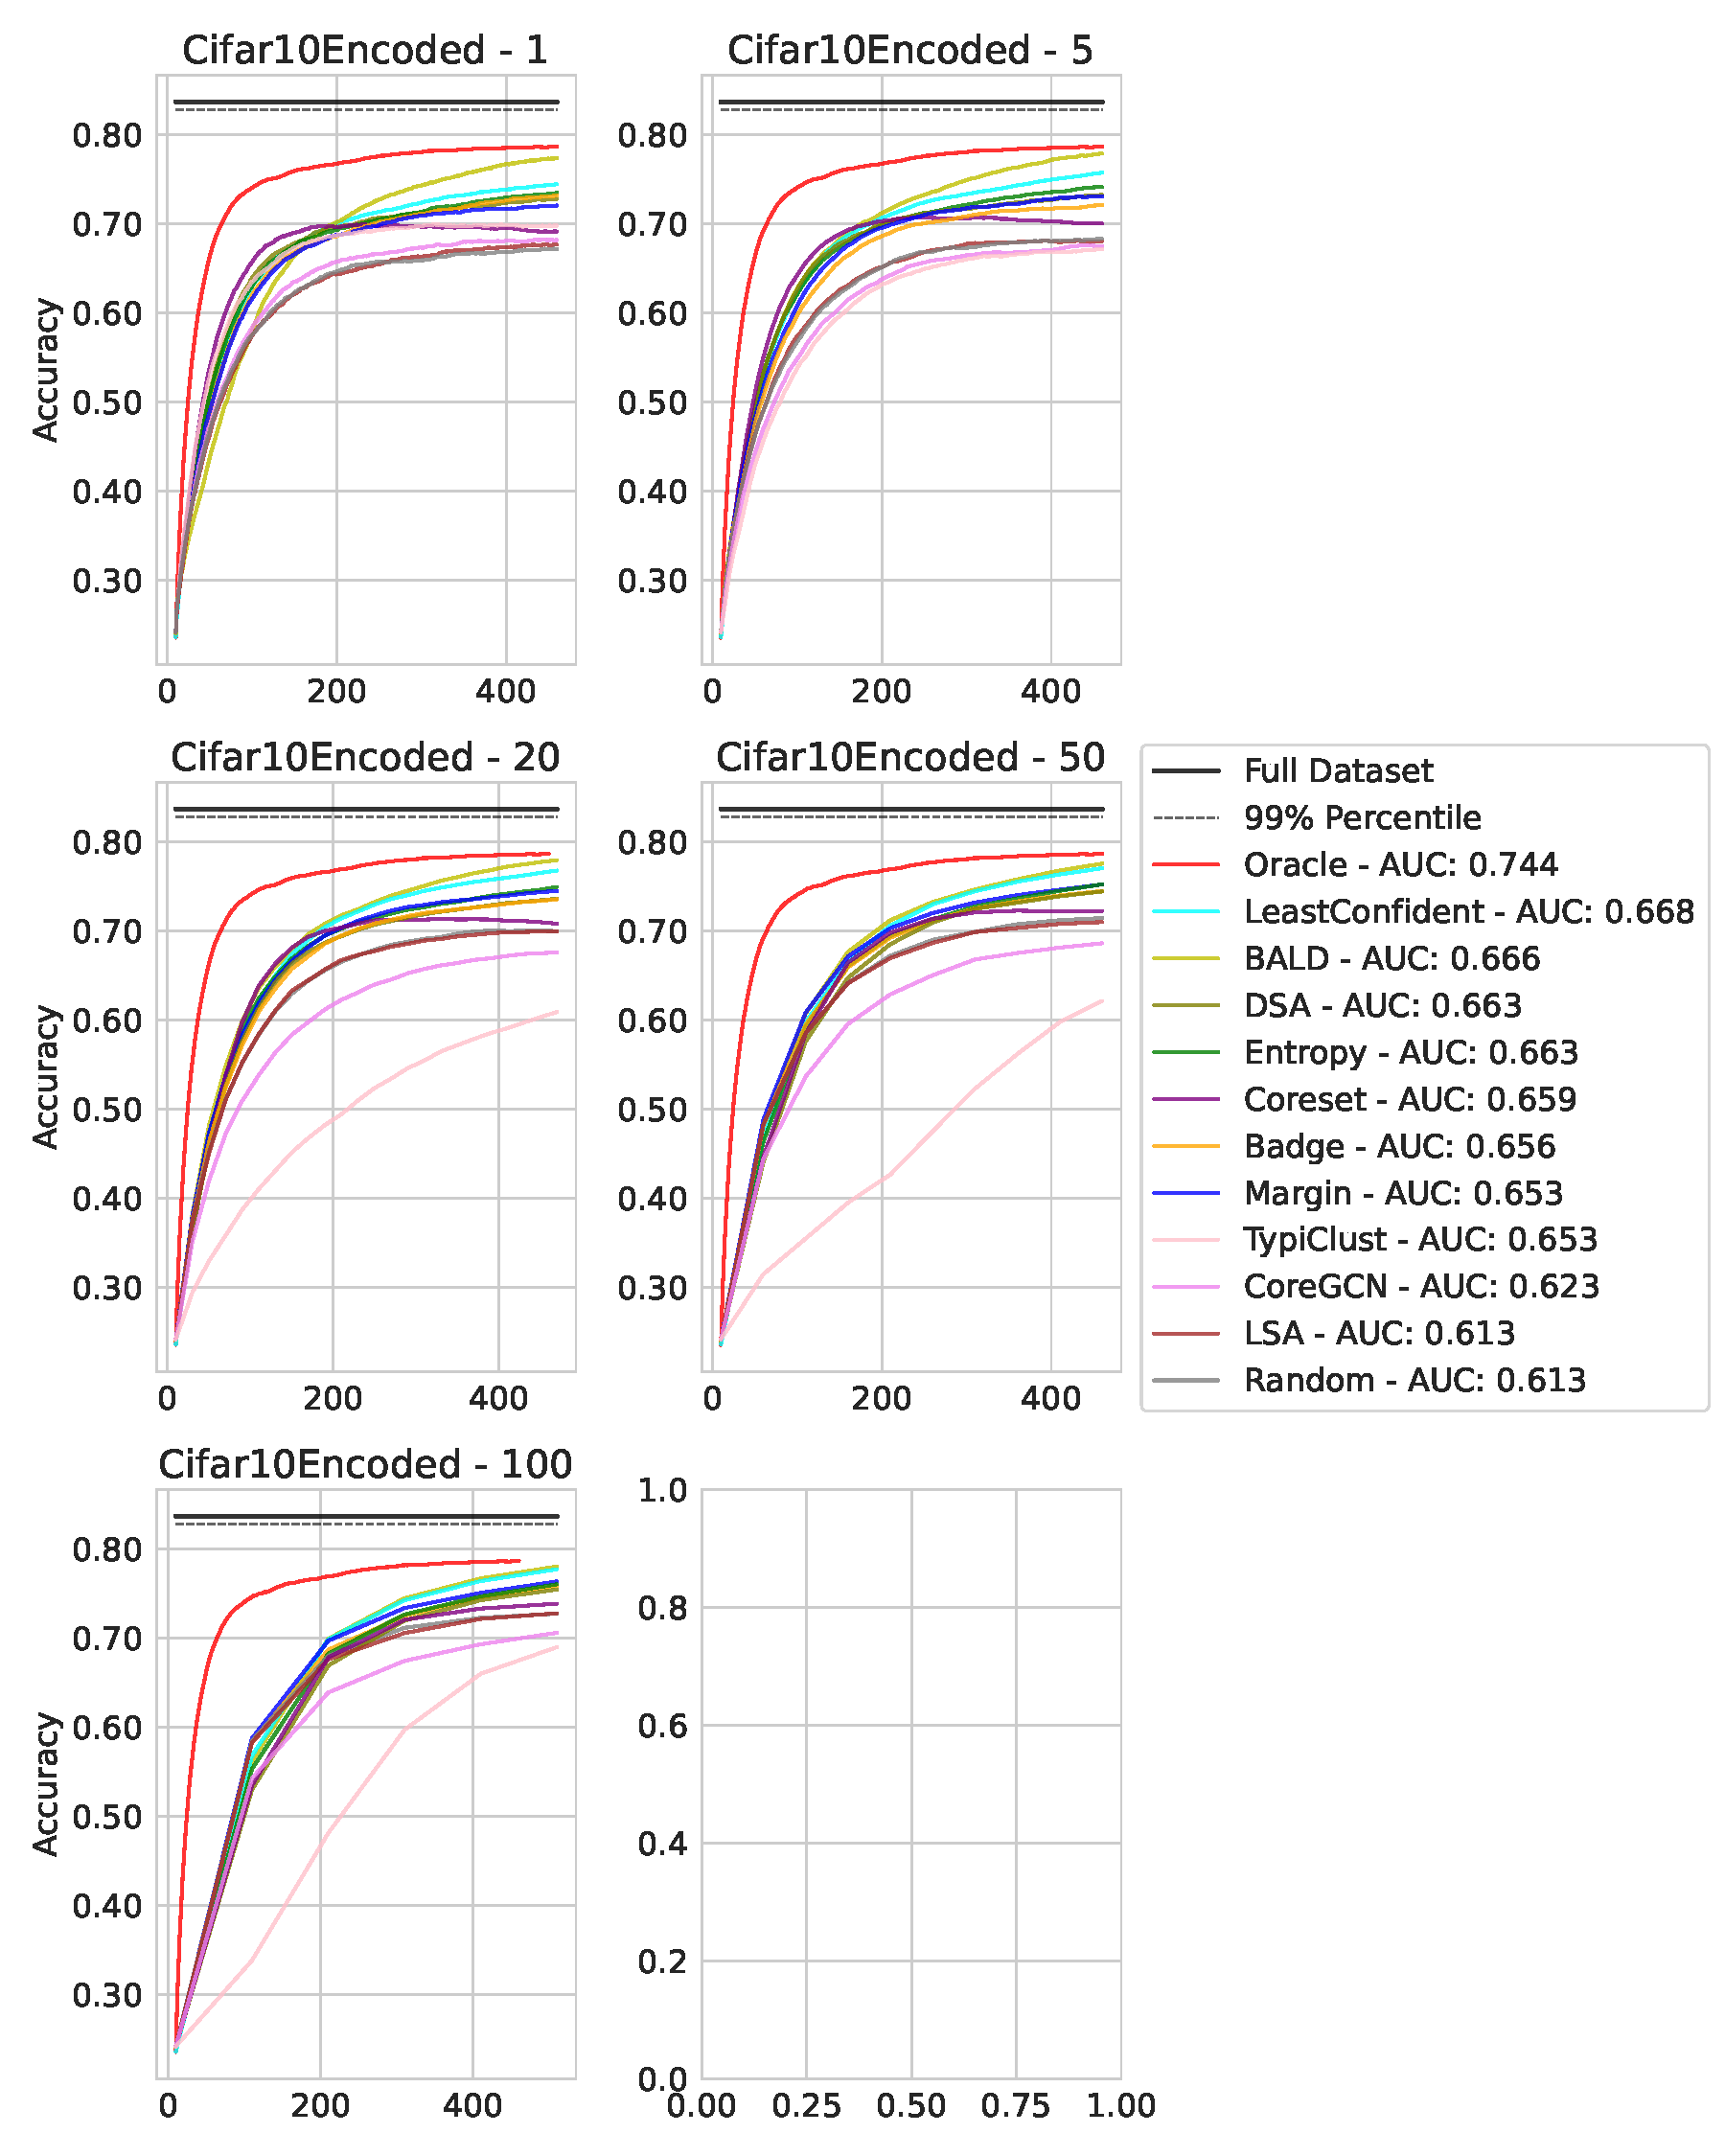
\includegraphics[width=0.49\linewidth]{img/eval_cifar10_enc} \\ [2mm]
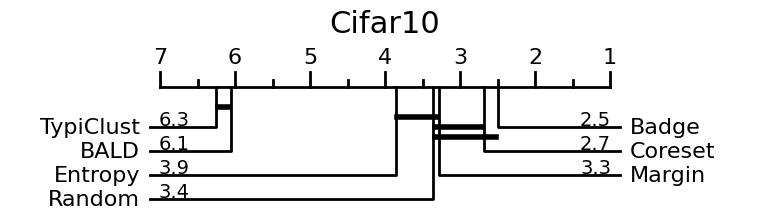
\includegraphics[width=0.49\linewidth]{img/micro_cifar10.jpg}
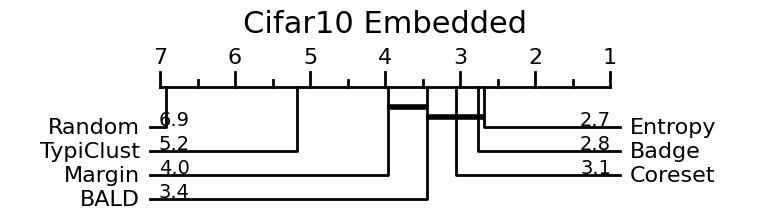
\includegraphics[width=0.49\linewidth]{img/micro_cifar10_enc.jpg} \\ [4mm]
\end{figure}
\begin{figure}[H]
\centering
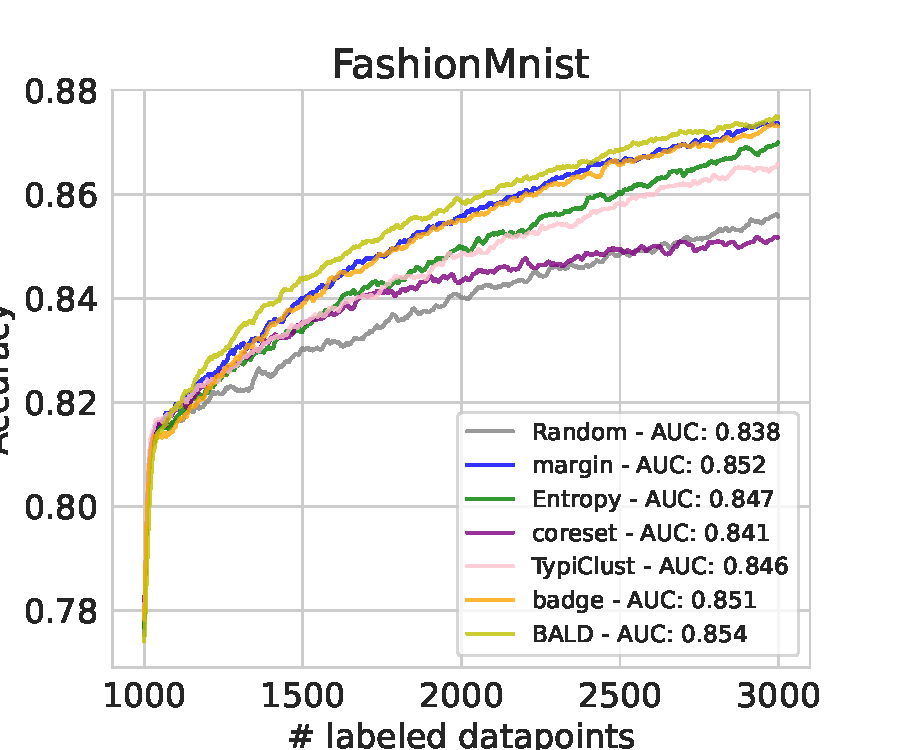
\includegraphics[width=0.49\linewidth]{img/eval_fmnist}
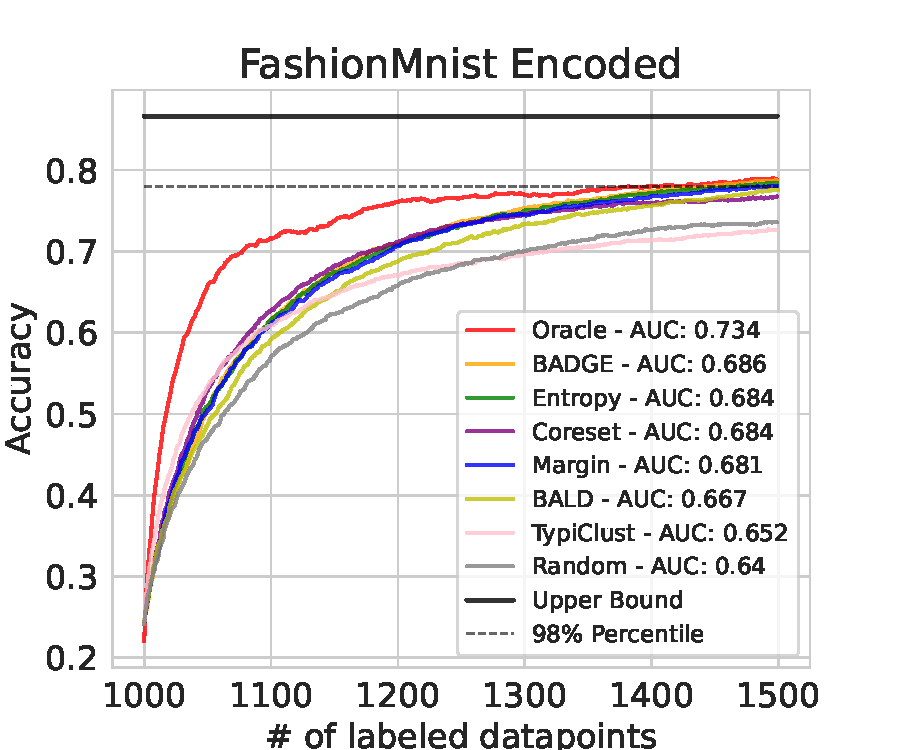
\includegraphics[width=0.49\linewidth]{img/eval_fmnist_enc} \\ [2mm]
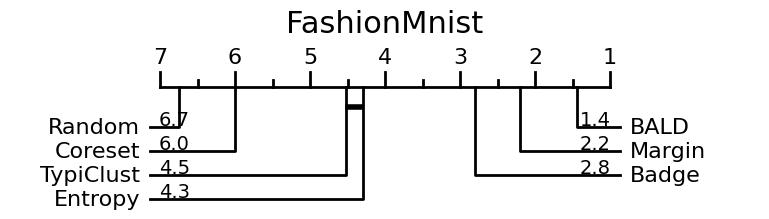
\includegraphics[width=0.49\linewidth]{img/micro_fmnist.jpg}
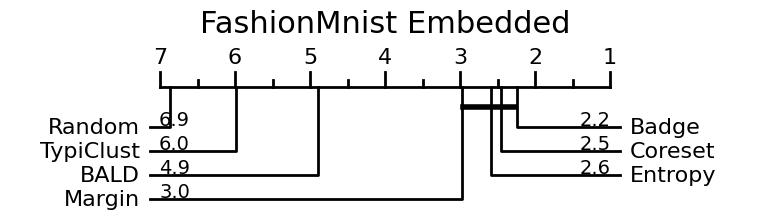
\includegraphics[width=0.49\linewidth]{img/micro_fmnist_enc.jpg} \\ [4mm]
\end{figure}
\begin{figure}[H]
\centering
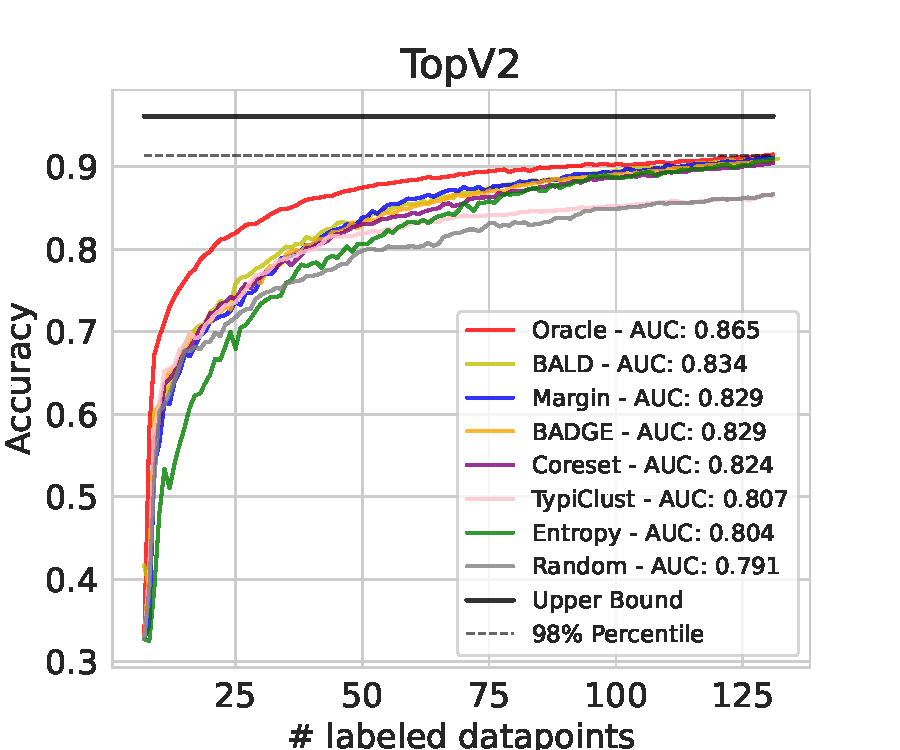
\includegraphics[width=0.49\linewidth]{img/eval_topv2}
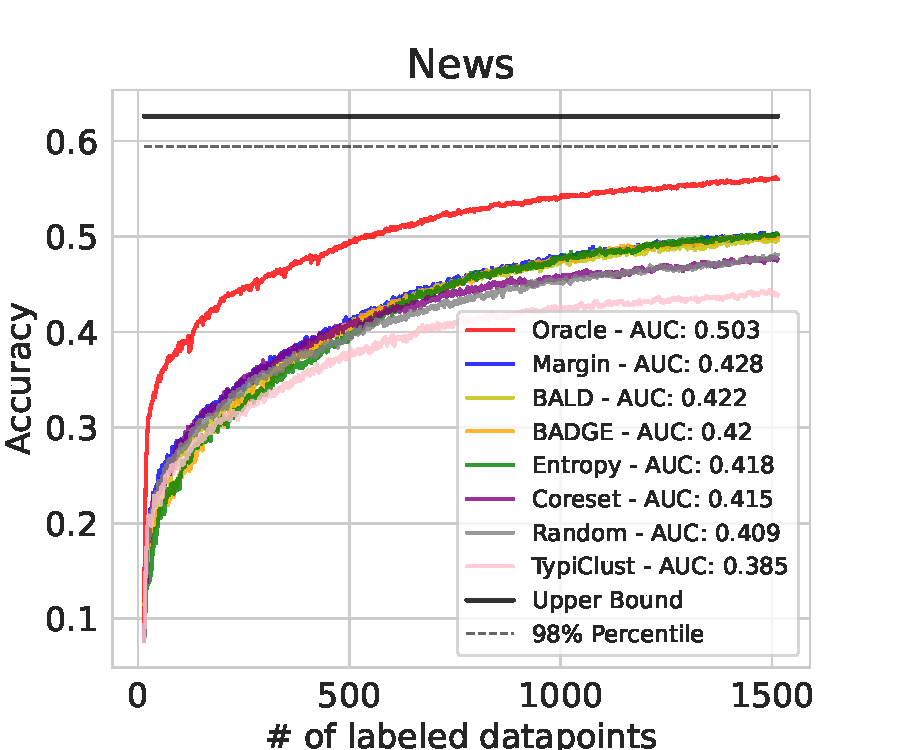
\includegraphics[width=0.49\linewidth]{img/eval_news} \\ [2mm]
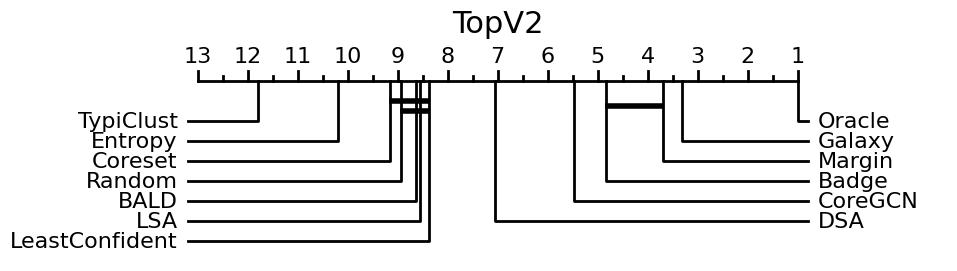
\includegraphics[width=0.49\linewidth]{img/micro_topv2.jpg}
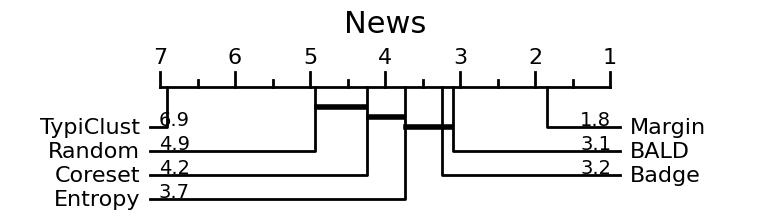
\includegraphics[width=0.49\linewidth]{img/micro_news.jpg} \\ [4mm]
\end{figure}


\section{Alternative Plot for Restarts Ablation}
\begin{figure}[H]
	\centering
	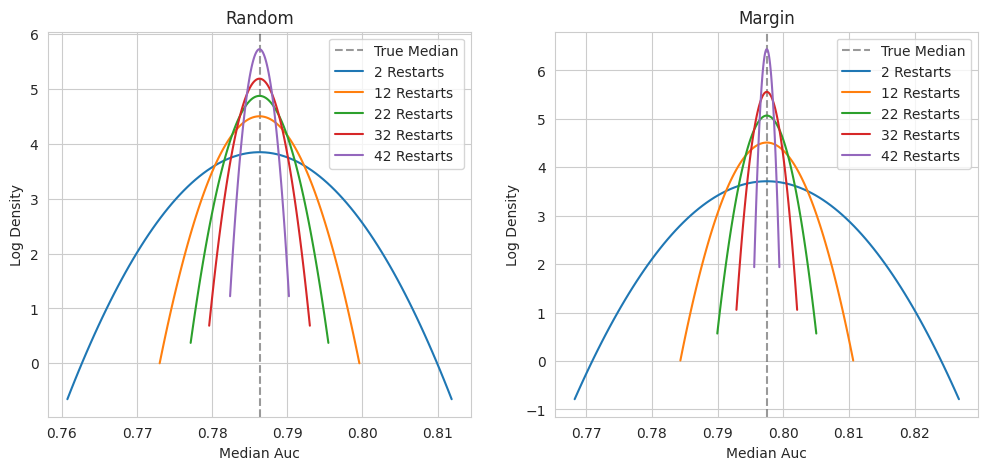
\includegraphics[width=\linewidth]{img/ablation_restarts_2}
\end{figure}

\section{Hyperparameters per AL Algorithm}\label{app:agent_hyperparameters}
\begin{table}[H]
	TODO
\end{table}

\section{Hyperparameters per Dataset}\label{app:hyperparameters}
\begin{table}[H]
	\centering
	\begin{tabular}{l || l | l l l l}
		Dataset & Classifier & Optimizer & LR & Weight Decay & Dropout \\
		\hline
		Splice & [24, 12] & NAdam & 1.2e-3 & 5.9e-5 & 0 \\
		SpliceEnc. & linear & NAdam & 6.2e-4 & 5.9e-6 & 0 \\
		DNA & [24, 12] & NAdam & 3.9e-2 & 3.6e-5 & 0 \\
		DNAEnc & linear & NAdam & 1.6e-3 & 4e-4 & 0 \\
		USPS & [24, 12] & Adam & 8.1e-3 & 1.5e-6 & 0 \\
		USPS & linear & NAdam & 7.8e-3 & 1.9e-6 & 0 \\
		FashionMnist & ResNet18 & NAdam & 1e-3 & 0 & 0 \\
		FashionMnistEnc & linear & Adam & 1.6e-3 & 1e-5 & 5e-2 \\
		Cifar10 & ResNet18 & NAdam & 1e-3 & 0 & 0 \\
		Cifar10Enc & linear & NAdam & 1.7e-3 & 2.3e-5 & 0 \\
		TopV2 & BiLSTM & NAdam & 1.5e-3 & 1.7e-7 & 5e-2 \\
		News & BiLSTM & NAdam & 1.5e-3 & 1.7e-7 & 5e-2 \\
	\end{tabular}
	\caption{Classifier architectures and optimized hyperparameters per dataset. Numbers in brackets signify a MLP with corresponding hidden layers.}
	\label{tab:architectures}
\end{table}

\section{Comparison of Different Classifier Sizes}\label{app:classifier_size}
We tested two different classifier sizes in Splice and DNA:
\begin{itemize}
	\item Small: [24, 12] (2400 parameters)
	\item Big: [24, 48, 48] (5700 parameters)
\end{itemize}
\begin{figure}
	\centering
	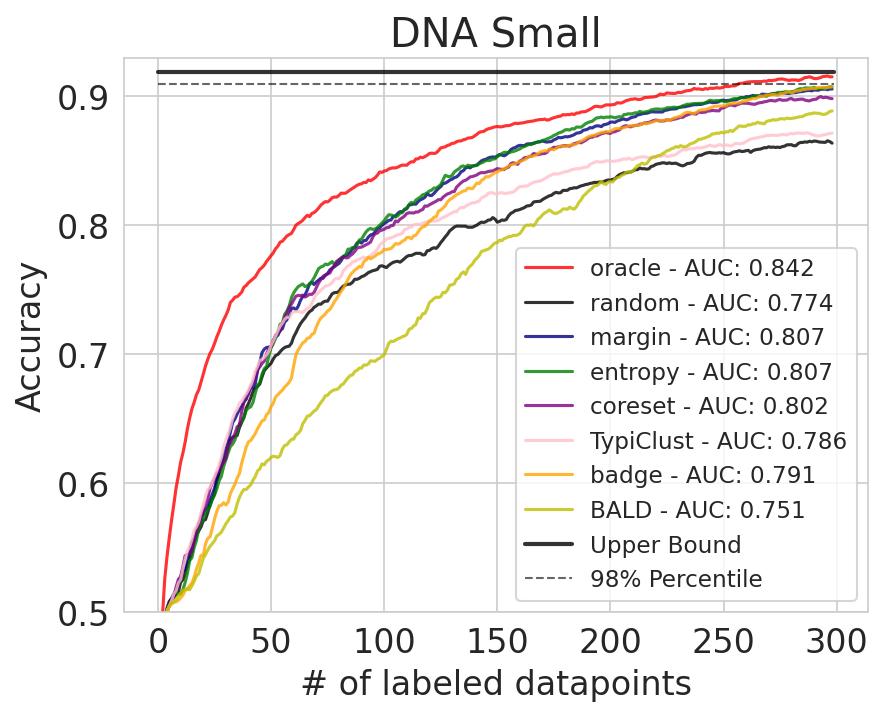
\includegraphics[width=0.49\linewidth]{img/supp_dna_small.png}
	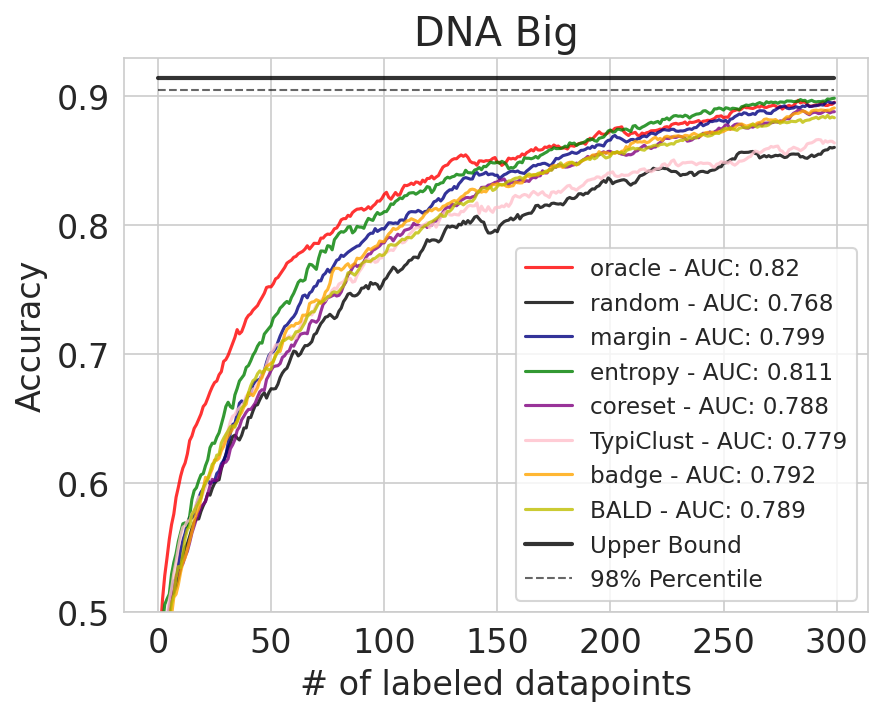
\includegraphics[width=0.49\linewidth]{img/supp_dna_big.png}
	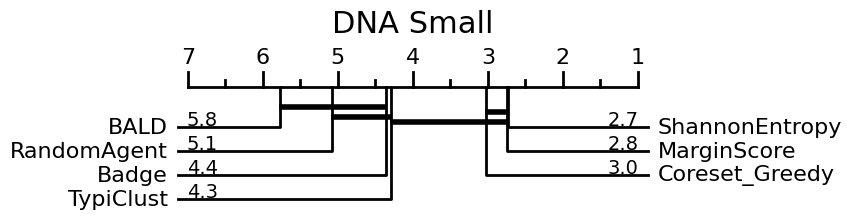
\includegraphics[width=0.49\linewidth]{img/supp_micro_dna_small.png}
	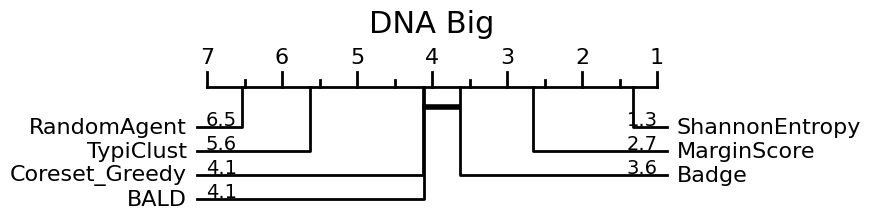
\includegraphics[width=0.49\linewidth]{img/supp_micro_dna_big.png}
	\caption{Comparison of small and big classifiers for the DNA dataset}
\end{figure}
\begin{figure}
	\centering
	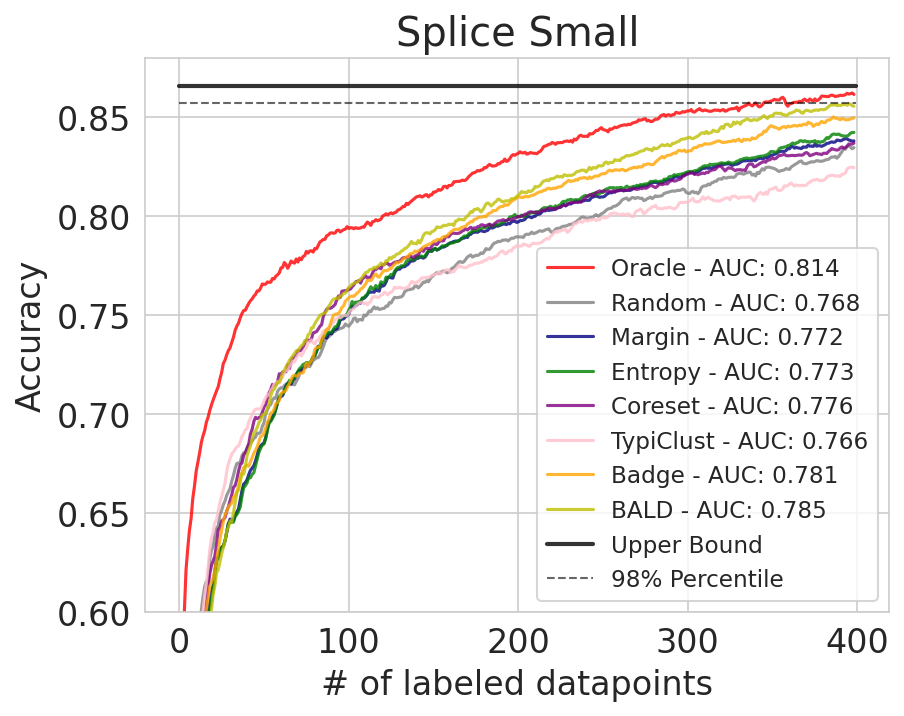
\includegraphics[width=0.49\linewidth]{img/supp_splice_small.png}
	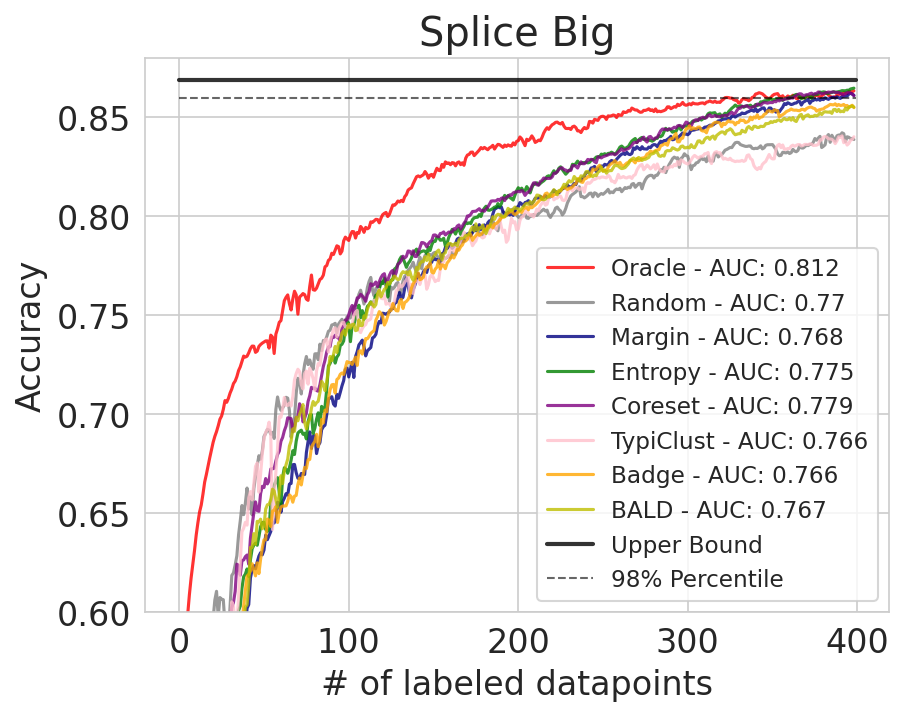
\includegraphics[width=0.49\linewidth]{img/supp_splice_big.png}
	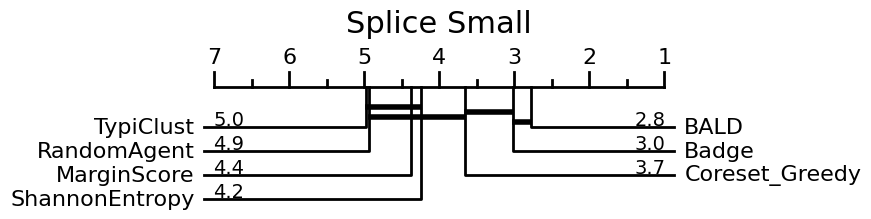
\includegraphics[width=0.49\linewidth]{img/supp_micro_splice_small.png}
	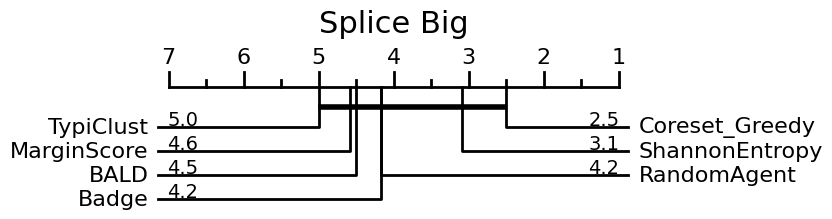
\includegraphics[width=0.49\linewidth]{img/supp_micro_splice_big.png}
	\caption{Comparison of small and big classifiers for the Splice dataset}
\end{figure}


\section{Comparison of different sample sizes}
\begin{figure}[H]
\centering
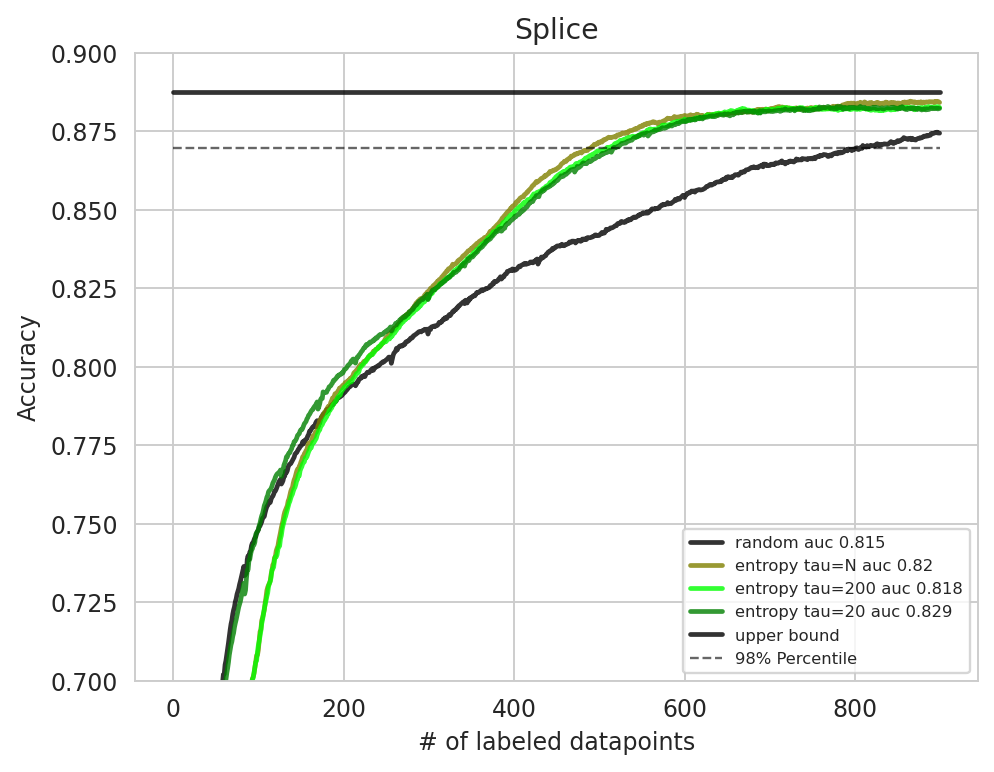
\includegraphics[width=0.7\linewidth]{img/tau_ablation.png}
\end{figure}

\section{AL Pseudocode}
\begin{algorithm}[H]
	\caption{Active Learning}\label{alg:active_learning}
	\begin{algorithmic}[1]
		\Require $\mathcal{U}$ \Comment{Unlabeled Pool}
		\Require $\tau$ \Comment{Unlabeled Sample Size}
		\Require $\Omega$ \Comment{AL Agent}
		\Require $\omega$ \Comment{Environment State function}
		\State $\mathcal{L}^{(1)} \gets \operatorname{seed}(\mathcal{U})$  \Comment{Create the initial labeled set}
		\State $\mathcal{U}^{(1)} \gets \mathcal{U}$
		\For{$i := 1 \ldots B$}
		\State $\text{acc}^{(i)} \gets \operatorname{Retrain}(\mathcal{L}^{(i)})$  %\Comment{$\operatorname{Retrain}(\mathcal{L}^{(i)})$ is shorthand for $\operatorname{Retrain}(\mathcal{L}^{(i)}, \mathcal{L}^\text{test}, \hat y_\theta, e^\text{max})$}
		%\State $u^{(i)} \sim \text{unif}(1:|\mathcal{U}^{(i)}|)$
		\State $a^{(i)} \gets \Omega(\mathcal{U}^{(i)}) \hspace{1mm};\hspace{2mm} a \in 1:|\mathcal{U}^{(i)}|$ 
		%\Comment{$a^{(i)}$ is an index inside of $u^{(i)}$}
		\State $y^{(i)} \gets \operatorname{label}(\mathcal{U}^{(i)}_{a})$ 
		%\Comment{$u^{(i)}_{a}$ is shorthand for $u^{(i)}_{a^{(i)}}$}
		\State $\mathcal{L}^{(i+1)} \gets \mathcal{L}^{(i)} \cup \{(\mathcal{U}^{(i)}_a, y^{(i)})\}$
		\State $\mathcal{U}^{(i+1)} \gets \mathcal{U}^{(i)} \setminus \{\mathcal{U}^{(i)}_a\}$
		\EndFor
		\State
		\Return $\frac{1}{B} \sum_{i=1}^{B} \text{acc}^{(i)}$
	\end{algorithmic}
\end{algorithm}

\begin{algorithm}[H]
	\caption{Retrain}\label{alg:retrain}
	\begin{algorithmic}[1]
		\Require $\mathcal{L}$ \Comment{Labeled Pool}
		\Require $\mathcal{D}_\text{val}$ \Comment{Validation Data}
		\Require $\mathcal{D}_\text{test}$ \Comment{Test Data}
		\Require $\hat y_\theta$ \Comment{Class. Model}
		\Require $e^\text{max}$ \Comment{Maximum Epochs}
		\State $\text{loss}^* \gets \infty$
		\For{$i := 1 \ldots e^{\text{max}}$}
		\State $\theta_{i+1} \gets \theta_i - \eta \nabla_\theta \ell(\mathcal{L}, \hat y_{\theta})$
		\State $\text{loss}_i \gets \ell(\mathcal{D}^\text{val}, \hat y_{\theta})$
		\If{$\text{loss}_i < \text{loss}^*$}
		\State $\text{loss}^* \gets \text{loss}_i$
		\Else
		\State Break
		\EndIf
		\EndFor
		\State
		\Return Acc($\mathcal{D}^\text{test}, \hat y_{\theta}$)
	\end{algorithmic}
\end{algorithm}

\end{document}
